\documentclass[journal=jacsnano,manuscript=article]{achemso}
\usepackage{chemformula} % Formula subscripts using \ch{}
\usepackage[T1]{fontenc} % Use modern font encodings
\usepackage{xr}
\usepackage{lineno}
\newcommand*\mycommand[1]{\texttt{\emph{#1}}}

\author{Ganesh Ghimire} 
\email{gangh@dtu.dk}
\affiliation{Department of Electrical and Photonics Engineering, Technical University of Denmark, Denmark}

\author{Rajesh Kumar Ulaganathan} 
\affiliation{1 Centre for Nanotechnology, Indian Institute of Technology Roorkee, 247667, India}

\author{Oleksii Ilchenko}
\affiliation{Department of Health Technology Nanoprobes, Technical University of Denmark, Denmark}
\alsoaffiliation{Lightnovo, 3460 Birkerod, Denmark}
\author{Denys I. Miakota}
\affiliation{Department of Electrical and Photonics Engineering, Technical University of Denmark, Denmark}

\author{Arias Juan Camilo} 
\affiliation{Department of Electronics and Nanoengineering, Aalto University, Espoo, Finland }

\author{Claudia Piccinini} 
\affiliation{Department of Electrical and Photonics Engineering, Technical University of Denmark, Denmark}


\author{Yurii Pilhun}
\affiliation{Lightnovo, Blokken 15, 1, tv. 3460 Birkerod, Denmark}

\author{Eunji Lee}
\affiliation{Department of Energy Science, Sungkyunkwan University, South Korea}

\author{Krishna P. Dhakal}
\affiliation{Department of Energy Science, Sungkyunkwan University,  South Korea}

\author{Jeongyong Kim}
\affiliation{Department of Energy Science, Sungkyunkwan University,  South Korea}

\author{Battulga Munkhbat} 
\affiliation{Department of Electrical and Photonics Engineering, Technical University of Denmark, Denmark}

\author{Sun Zhipei} 
\affiliation{Department of Electronics and Nanoengineering, Aalto University, Espoo, Finland }
\author{Stela Canulescu}
\affiliation{Department of Electrical and Photonics Engineering, Technical University of Denmark, Denmark}
\email{stec@dtu.dk}

\title{Polarization sensitive photodetection and anisotropic optical response in \ch{MoS2} nanoribbons }
\abbreviations{IR,NMR,UV}
\keywords{Pulsed Laser Deposition, STEM, DFT}

%%%%%%%%%%%%%%%%%%%%%%%%%%%%%%%%%%%%%%%%%%%%%%%%%%%%%%%%%%%%%%%%%%%%%
%%%%%%%%%%%%%%%%%%%%%%%%%%%%%%%%%%%%%%%%%%%%%%%%%%%%%%%%%%%%%%%%%%%%%
\begin{document}
\newpage
\begin{abstract}
The symmetry-dependent properties of multilayer \ch{MoS2} give rise to rich electron–phonon interactions, and structural perturbations can strongly modify these couplings beyond those expected in conventional 2H-stacked crystals. Here, we systematically investigate the polarization-dependent Raman response, differential reflectance, and photodetection characteristics of \ch{MoS2} nanoribbons synthesized via a two-step process that combines pulsed laser deposition and sulfurization. The nanoribbons exhibit pronounced polarization anisotropy in all three measurements, in stark contrast to the isotropic behavior observed in 2D triangular \ch{MoS2} grown under identical conditions. We attribute the emerging anisotropy in the nanoribbons to their distinct stacking configuration, predominantly 3R rather than 2H, which modifies the vibrational and electronic symmetry and manifests in both optical and electrical responses. The robust anisotropic Raman signatures, angle-dependent excitonic absorption, and polarization-sensitive photocurrent, where the cross-polarized photocurrent exceeds the parallel configuration by a factor of 1.5, highlight the unique optoelectronic properties enabled by reduced dimensionality and altered stacking order. The synthesis of stable, anisotropic \ch{MoS2} nanoribbons opens new avenues for polarization-sensitive and directionally engineered optoelectronic devices.
\end{abstract}

\section{Introduction}

Two-dimensional (2D) transition metal dichalcogenides (TMDs) have emerged as a versatile platform for optoelectronic, photonic, and quantum technologies owing to their tunable band structures, strong excitonic resonances, and light–matter interactions.\cite{Zhang2019, Zhang2020} Beyond phase and layer number, the micro- and nanostructure of TMD domains plays a decisive role in determining their physical properties. Variations in crystallite size, edge configuration, shape, and dimensionality profoundly influence catalytic activity, mechanical flexibility, optical selection rules, and quantum behavior.\cite{XZhang2019CVD2D, XZhang2021HTS2D, QiangVLSWS22021} Conventional growth using chemical vapor deposition (CVD) typically produces isotropic triangular monolayers through omnidirectional lateral growth. However, many desirable attributes, such as enhanced edge reactivity, tunable strain fields, quantum confinement, and directional carrier transport, become increasingly pronounced as TMDs approach the one-dimensional (1D) limit. Indeed, transitioning from 2D layers to 1D nanoribbons (NRs) introduces strong lateral confinement and dramatically increases the edge-to-area ratio, enabling electronic and magnetic phenomena that are inaccessible in isotropic sheets. Theoretical studies predict that TMD NRs exhibit width-dependent band gaps,\cite{Dolui2012} metal–insulator transitions,\cite{He2017} enhanced thermoelectric efficiency\cite{Zhang2016}, and spin- or valley-polarized edge states.\cite{Cheng2017} Realizing these effects experimentally requires precise control over NR width, edge termination, and crystallographic coherence. Recent studies have therefore focused on synthesis strategies that break in-plane symmetry, including ledge-guided epitaxy, vapor–liquid–solid growth, and anisotropic CVD on crystalline substrates such as Ge(001) or sapphire.\cite{Aljarb2020, Li2021}. Substrate-directed approaches provide a powerful route to shape-engineered TMDs. For example, MoS\(_2\) nanoribbons grown on PH\(_3\)-functionalized Si(001) exhibit widths tunable from 50–430~nm and show a characteristic $\sim$50~meV photoluminescence (PL) blue shift due to lateral exciton confinement\cite{ChowdhuryNature}. The surface Si–P and P–P dimers formed during PH\(_3\) dissociation mediate highly anisotropic nucleation and directional edge propagation. This strategy extends to MoSe\(_2\), where the ribbon width depends on the H\(_2\) partial pressure, reflecting hydrogen-driven modification of Si–P surface dimers.\cite{ChowdhuryNature}. Carbon nanotubes (CNTs) have been widely explored as hosts for TMD chains and ribbons,\cite{Tanaka2025,Miakota2023MoS2NR,G_Ghimire}, but their intrinsic electronic states complicate direct optical interrogation. Boron nitride nanotubes, with their wide ($\sim$5.5~eV) and diameter-independent bandgap, provide an inert environment in which few-nanometer MoS\(_2\) ribbons display zigzag-edge structures, compressive strain, and pronounced optical anisotropy revealed through angle-resolved polarized Raman spectroscopy.\cite{Tanaka2025}

In this work, we show that () MoS$_2$ nanoribbons exhibit pronounced anisotropy across vibrational, optical, and optoelectronic responses. In contrast to conventional MoS$_2$ monolayers, which exhibit in-plane isotropy due to their hexagonal symmetry, the nanoribbons show strong polarization dependence arising from reduced dimensionality and symmetry breaking. Specifically, angle-resolved Raman spectroscopy reveals a distinct twofold symmetry in both A$_{1g}$ and E$^1_{2g}$ modes, indicating anisotropic lattice dynamics and modified electron--phonon interactions.

Furthermore, polarization-resolved differential reflectance measurements uncover directionally modulated excitonic transitions, with enhanced anisotropy in higher-energy and cavity-coupled modes, highlighting the critical role of  confinement in governing light--matter interactions. Importantly, this intrinsic anisotropy directly translates into device functionality. Photodetectors based on MoS$_2$ nanoribbons exhibit strongly polarization-sensitive photocurrent with pronounced directional dependence in photocarrier generation and transport, demonstrating their potential for polarization-selective optoelectronic applications.

\section{Results and discussion}

The \ch{MoS2} nanoribbons were synthesized using a chemical vapor deposition system, as illustrated in Fig.~\ref{fig:synthesis_schematic}, with the key distinction that solid thin-film precursors were employed in this process instead of powder precursors in a standard CVD process. The precursors consist of a \ch{MoO_{3-x}} thin film deposited by pulsed laser deposition (PLD) and subsequently coated with a NaF layer. Upon heating to 800~\textdegree C, the NaF reacts with the oxide film to form a transient Na--Mo--O liquid phase. Meanwhile, sulfur powder placed upstream in a separately heated zone releases sulfur vapor, which is continuously transported to the reaction zone by the carrier gas (Ar/5\% H\textsubscript{2}). 
When sulfur species dissolve into the liquid Na--Mo--O droplets, a vapor--liquid--solid (VLS) conversion process is initiated. During this process, the reaction between sulfur and the Na--Mo--O droplets leads to the formation of a \ch{MoS2} layer. The emergence of this layer modifies the local surface and interfacial energies, resulting in asymmetric wetting conditions that induce the droplet to crawl across the substrate. As the droplet moves, it continuously mediates the conversion of the oxide precursor into \ch{MoS2}, eventually resulting in solidification. Consequently, the liquid phase acts as a catalytic medium that directs the unidirectional growth of \ch{MoS2} nanoribbons, rather than the isotropic 2D platelets typically formed during conventional \ch{MoS2} growth~\cite{G_Ghimire, Miakota2023MoS2NR}. As shown in Fig.~\ref{fig:synthesis_schematic}b and Fig.~\ref{fig:si_6_width_dependent_anisotropy_wider}, the length of the \ch{MoS2} nanoribbons is usually in the range of 10 micrometers, and the width  up to 500 nm, exhibiting
a high anisotropic ratio.


\begin{figure}[ht!]
    \centering
    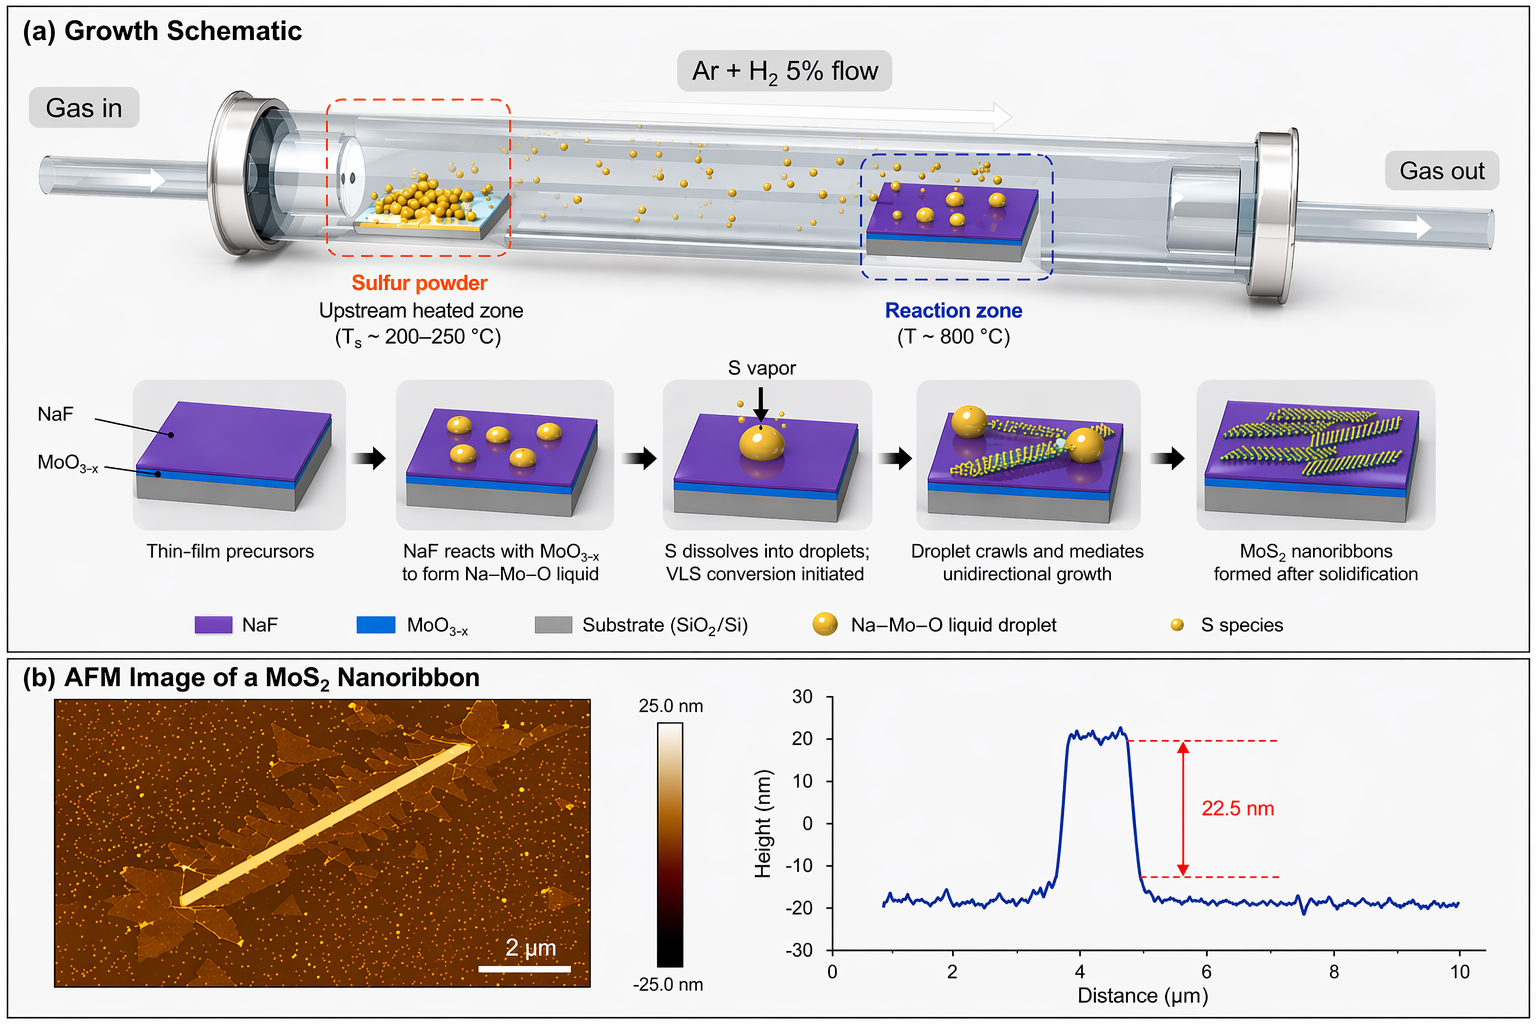
\includegraphics[width=1.0\linewidth]{Figures/Figure_1.jpeg.png}
    \caption{
    \textbf{Synthesis of MoS$_2$ nanoribbons.}
    (a) Schematic of the CVD growth process, where sulfur vapor reacts with a NaF/MoO$_3$ precursor under an Ar/H$_2$ (5\%) flow to form MoS$_2$ nanoribbons. 
    (b) AFM image of a typical MoS$_2$ nanoribbon, exhibiting a length-to-width ratio of $\sim$10. 
    (c) Corresponding height profile showing a nanoribbon thickness of $\sim$22.5 nm.}
    \label{fig:synthesis_schematic}
\end{figure}

To probe the anisotropy of the MoS$_2$ nanoribbons, we performed polarization-resolved Raman microscopy (PRM) mapping using a Single-Acquisition Raman Orientation Mapping (SAROM) configuration. In this approach, the laser beam excites the sample with a defined polarization, and the scattered light is simultaneously analyzed across multiple polarization channels. As illustrated in Fig.~\ref{fig:Raman_2pol}a, the incident polarization is set to either $I{45}$ or $I_{135}$, while the scattered signal is detected along orthogonal directions $O_{45}$ and $O_{135}$. Representative PRM maps for both nanoribbons and triangular MoS$_2$ are shown in Fig.~\ref{fig:Raman_2pol}b.

The triangular MoS$_2$ monolayers exhibit nearly identical Raman intensities across all polarization channels, consistent with the isotropic vibrational response expected for the hexagonal 2H phase. In contrast, the nanoribbons show pronounced polarization-dependent variations in both A${1g}$ and E$^{1}{2g}$ modes, directly evidencing anisotropy. In particular, the E$^{1}{2g}$ mode intensity decreases significantly when the polarization changes from parallel to perpendicular with respect to the ribbon axis. The anisotropy ratio $(I_{\parallel}-I_{\perp})/(I_{\parallel}+I_{\perp})$ is clearly non-zero for both modes and is strongest for the A$_{1g}$ mode, reflecting its sensitivity to interlayer interactions and stacking configuration.

This behavior can be understood within the framework of Raman polarization selection rules, where the measured intensity depends on the orientation of the light polarization relative to the crystal symmetry and the phonon Raman tensor. In monolayer MoS$2$, the high in-plane symmetry leads to an essentially isotropic response, with the E$^{1}{2g}$ mode remaining angle-independent and the A$_{1g}$ mode showing only weak modulation. In contrast, the nanoribbons exhibit strong intrinsic anisotropy due to their quasi-one-dimensional geometry, which breaks the in-plane symmetry and introduces a preferred crystallographic direction along the ribbon axis.

The intrinsic nature of this anisotropy is further confirmed by polarization-dependent Raman measurements under sample rotation (Fig.~\ref{fig:schematic sample rotation}). In this configuration, the incident and analyzed polarizations are kept parallel while the sample is rotated, ensuring that the rotation angle directly reflects the crystallographic orientation. As shown in Fig.~\ref{fig:si_Mo_ribbon-Sample rotation} and Fig.~\ref{fig:si_2D_Triangular MoS2}, the nanoribbons display clear angular modulation in both A${1g}$ and E$^{1}{2g}$ modes, whereas the triangular monolayer remains largely isotropic, with modulation observed only in the A$_{1g}$ mode. The strong agreement between PRM mapping and rotation measurements confirms that the observed anisotropy is intrinsic to the nanoribbons and not an artifact of the measurement configuration.

A direct comparison between triangular monolayers and nanoribbons further highlights the role of dimensionality. As illustrated in Fig.~\ref{fig:raman_anisotropy}, the triangular monolayer retains the isotropic response characteristic of the 2H phase, with the E$^{1}_{2g}$ mode remaining nearly constant under rotation. In contrast, the nanoribbons exhibit a pronounced twofold angular dependence in both Raman modes, with maximum intensity when the polarization is aligned along the ribbon axis and minimum intensity when perpendicular. This strong anisotropy indicates a significant modification of the effective Raman tensor.

Structural analysis suggests that this behavior originates from symmetry-lowering effects in the nanoribbons, including quasi-1D confinement, 3R-like stacking, directional strain, and edge-induced distortions. These factors modify the vibrational environment and enhance the contrast between modes aligned parallel and perpendicular to the ribbon axis. Consequently, polarization-dependent Raman scattering emerges as a robust fingerprint of broken in-plane symmetry in MoS$2$ nanostructures. The pronounced anisotropy of both A${1g}$ and E$^{1}_{2g}$ modes reflects the reduced dimensionality and altered bonding environment, providing a sensitive probe of the structural and electronic anisotropy in these systems.

 



\begin{figure}
    \centering
    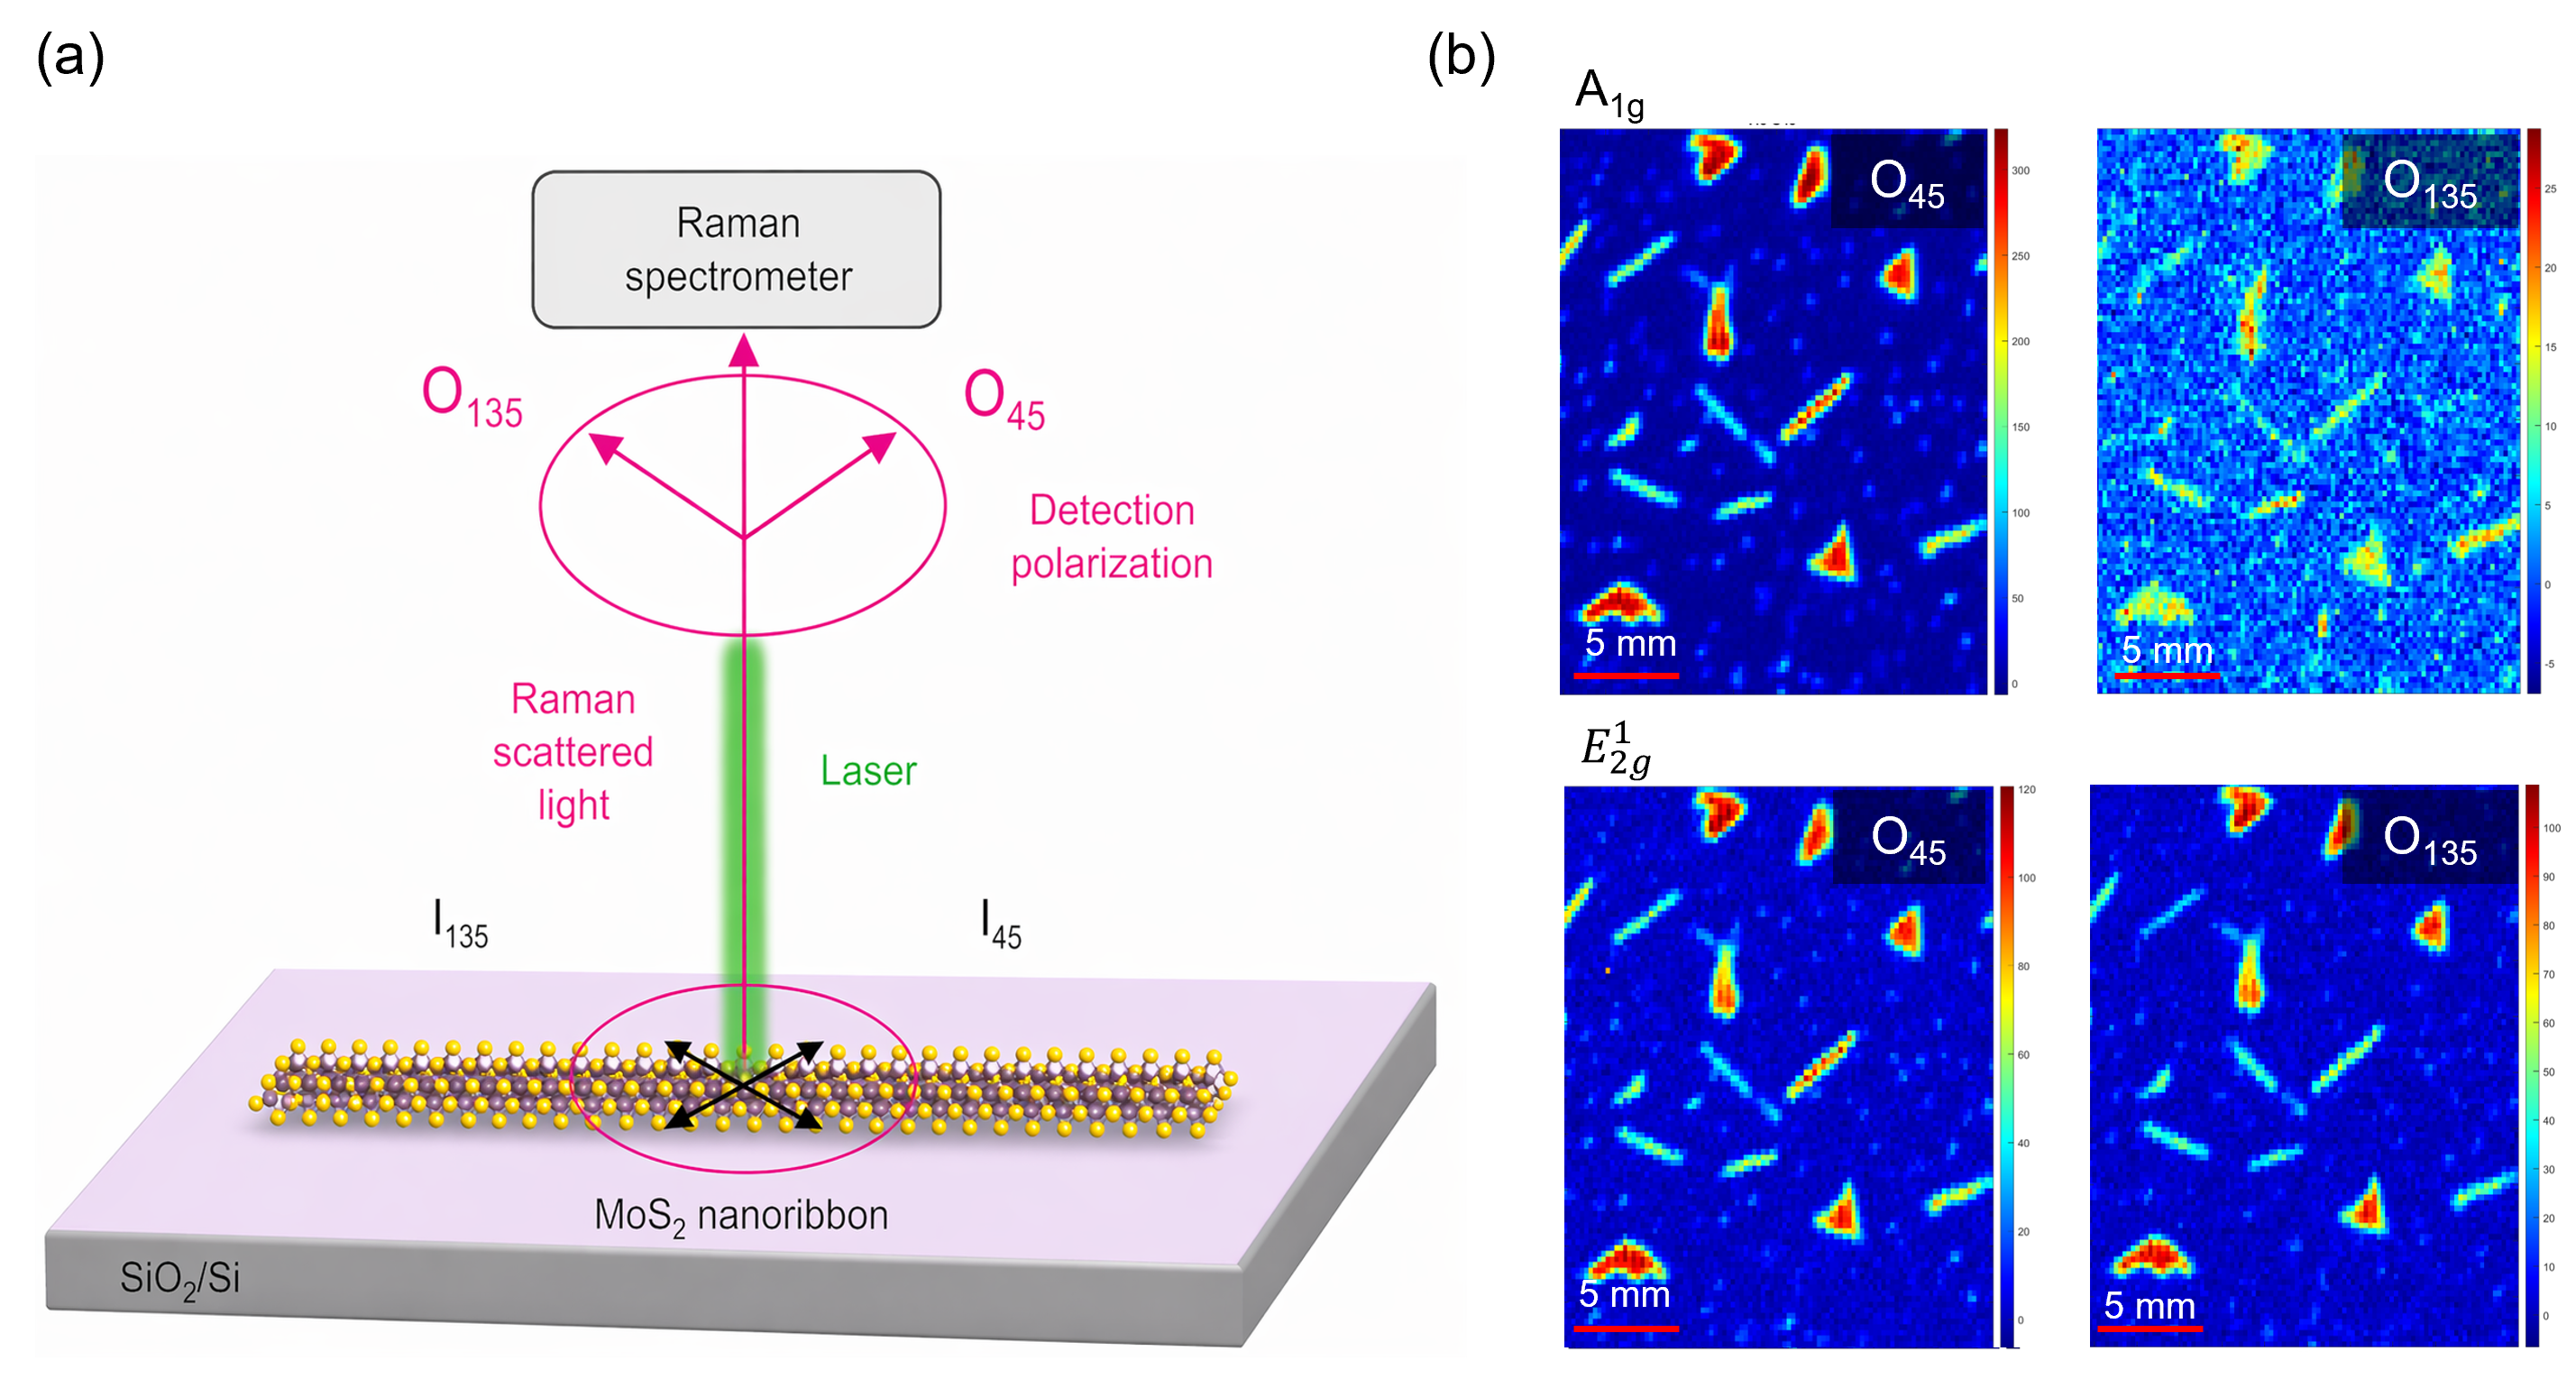
\includegraphics[width=1\linewidth]{Figures/Figure_2.png}
\caption{\textbf{Polarization-resolved Raman mapping of MoS$_2$ nanoribbons.}
(a) Schematic illustration of the polarization-resolved Raman measurement geometry, showing the incident laser polarization (I$_{45}$, I$_{135}$) and detection polarization (O$_{45}$, O$_{135}$) configurations. (b) Raman intensity maps of  A$_{1g}$ and E$^{1}_{2g}$ modes of MoS$_2$ acquired under different polarization configurations. The arrows above each map indicate the analyzed polarization direction.  Scale bars: 5~µm}
  \label{fig:Raman_2pol}
\end{figure}
.

\begin{figure}
    \centering 
    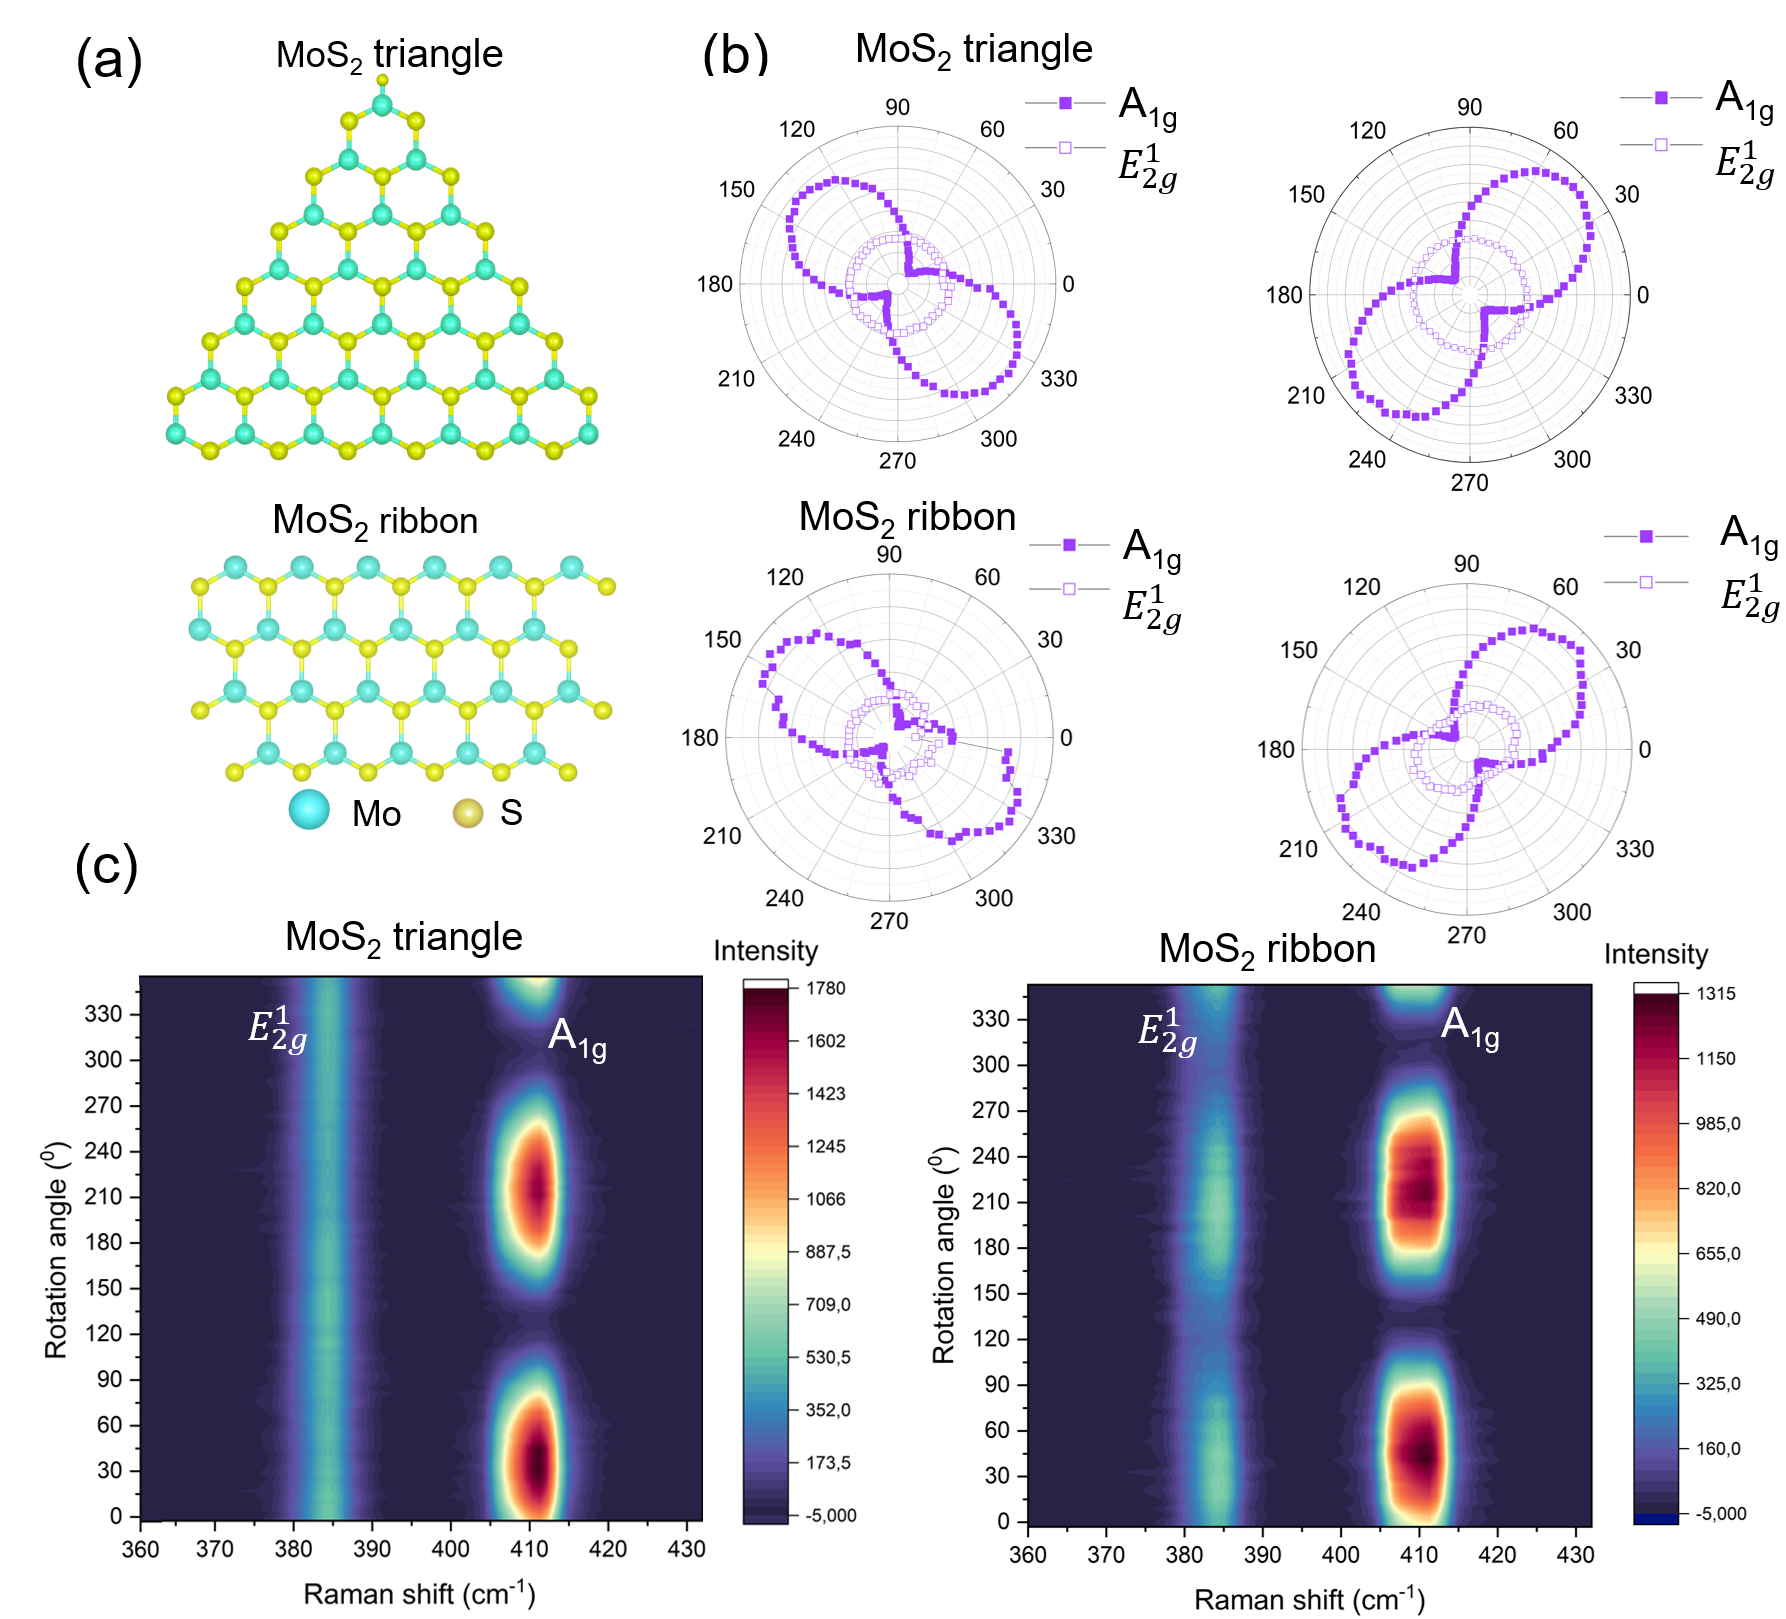
\includegraphics[width=0.9\linewidth]{Figures/Figure_3.png}
   \caption{
\textbf{Polarization-resolved Raman analysis of MoS$_2$ triangles and nanoribbons.}
(a) Atomic models of a monolayer \ch{MoS2} triangular flake (top) and a \ch{MoS2} nanoribbon (bottom). 
(b) Polar plots of the Raman intensities for the \ch{A_{1g}} and \ch{E^1_{2g}} Raman modes of the triangle (top) and ribbon (bottom) geometries. 
(c) Angle-resolved Raman contour maps of the triangular flake (left) and nanoribbon (right), where the color scale represents Raman intensity as a function of rotation angle and Raman shift. The $E_{2g}^{1}$ and $A_{1g}$ modes are indicated, highlighting the nearly isotropic response of the triangle compared to the pronounced anisotropy observed in the nanoribbon.}
\label{fig:raman_anisotropy}
\end{figure}



Second harmonic generation (SHG) provides a sensitive probe of inversion symmetry breaking, stacking order, and crystalline orientation in layered TMDs. While SHG has been widely explored in 2D \ch{MoS2} crystals, reports on  \ch{MoS2} nanoribbons remain limited. To investigate the non linear optical properties of our nanoribbons, we performed polarization resolved SHG imaging using an 800 nm pulsed excitation source in a backscattering configuration. Representative SHG maps are shown in Figure~\ref{fig:SHG}.
\begin{figure}%[htb]
    \centering
    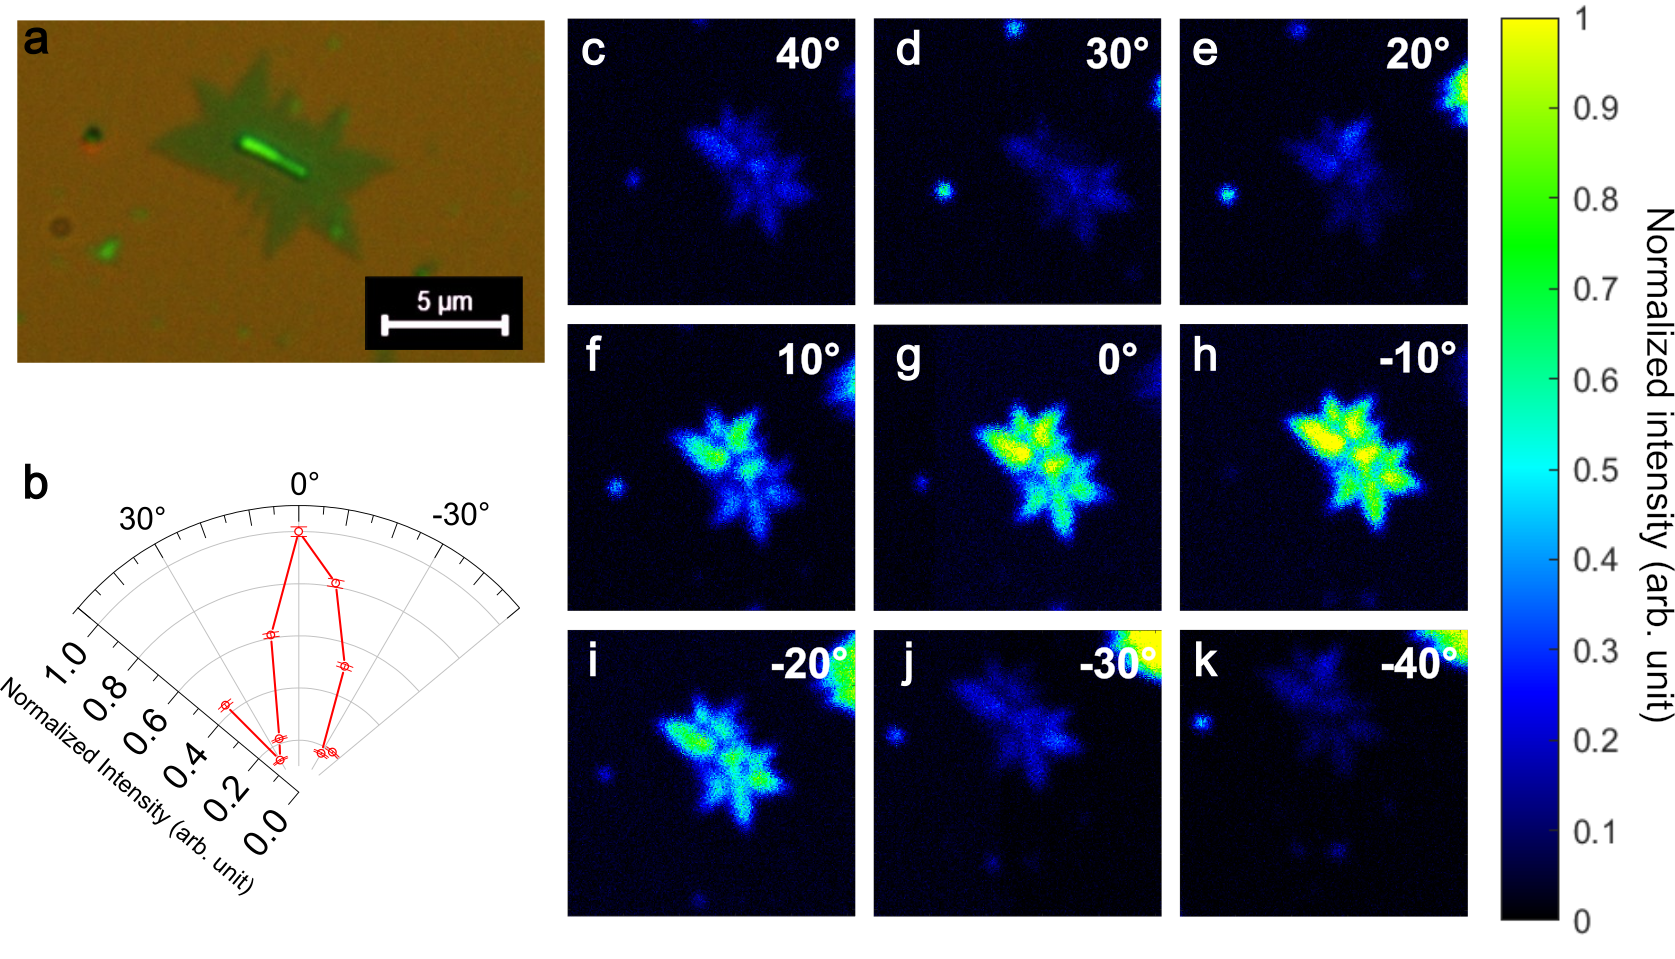
\includegraphics[width=1.0\linewidth]{Figures/Figure_5.png}
    \caption{\textbf{Polarization-dependent second harmonic generation (SHG) imaging of the \ch{MoS2} nanoribbons} 
    (a) Optical microscopy image of the star-shaped microflake with a \ch{MoS2} nanoribbon at its center.
    (b) Polar plot of the SHG intensity as a function of polarization angle (c–k). The plot is simplified to show only two minima and one maximum. 
    (c–k) SHG micrographs at different incident linear polarizations. The color bar represents normalized SHG intensity (arb. units). The linear polarizer is aligned parallel, yielding maximum intensity between $0^\circ$ and $-10^\circ$.}
    \label{fig:SHG}
\end{figure}
The optical microscope image in Figure~\ref{fig:SHG}a displays a well-defined \ch{MoS2} nanoribbon surrounded by a monolayer flake. Across varying incident polarization angles (Figures~\ref{fig:SHG}c--k), the SHG emission exhibits a clear angular modulation. As the pump polarization is rotated from $+40^\circ$ to $-40^\circ$, the SHG intensity from the star-shaped flake varies periodically, producing alternating bright and dim regions that reflect the underlying crystal symmetry. The strongest emission occurs near $0^\circ$ and $-10^\circ$, corresponding to excitation aligned with the armchair direction of the lattice, where efficient coupling to the nonlinear polarization of \ch{MoS2} maximizes SHG. In contrast, orientations near $\pm 30$^\circ$ suppress the SHG signal, consistent with symmetry-forbidden directions predicted for non-centrosymmetric trigonal prismatic lattices. The SHG polar plot in Figure~\ref{fig:SHG}b further reveals the characteristic six-fold rotational symmetry associated with the D$_{3h}$ lattice of monolayer \ch{MoS2}. This symmetry is preserved in the thin active region of the nanoribbon, demonstrating that the nanoribbon inherits the intrinsic crystalline orientation of the parent monolayer. The observed angular dependence follows the expected $I_{\mathrm{SHG}} \propto \cos^{2}(3\theta)$ behavior, confirming that the nonlinear susceptibility tensor maintains the same rotational symmetry as in monolayer \ch{MoS2}. Moreover, the intensity modulation matches the known thickness dependence of non-centrosymmetric \ch{MoS2}, indicating that the SHG response remains sensitive to local structural variations within the ribbon. The high SHG intensity across all measured orientations aligns with the expected behavior of 3R-\ch{MoS2}, which maintains broken inversion symmetry regardless of thickness. The thickness of the nanoribbons, derived from the AFM measurements (20 nm), falls within the reported band I regime of 3R \ch{MoS2}, where SHG intensity is known to be significantly enhanced~\cite{Shi2017}. This indicates that the nanoribbons crystallize in the 3R phase rather than the centrosymmetric 2H phase.
%We performed polarization-dependent Raman mapping to understand the observed Raman anisotropy on \ch{MoS2} nanoribbons together with 2D triangular \ch{MoS2}, as shown in ~Fig.~\ref{fig:raman_anisotropy} and ~Fig.~\ref {Fig_SI_4}. The vibrational response of the MoS$_2$ nanoribbons was against that of conventional 2D triangular monolayers using polarization-resolved Raman spectroscopy. ~Fig.~\ref{fig:raman_anisotropy}a sketches the atomic structure of a monolayer triangular flake and a nanoribbon, highlighting the transition from an isotropic hexagonal lattice to a laterally confined geometry with broken in plane symmetry. For the triangular monolayer, the angle-dependent Raman maps in~Fig.~\ref{fig:raman_anisotropy}c and the corresponding polar plots in ~Fig.~\ref{fig:raman_anisotropy}b (left) show the expected behavior of 2H–MoS$_2$. The in-plane E$^{1}_{2g}$ mode is essentially isotropic: its intensity remains nearly constant as the crystal is rotated, consistent with the threefold rotational symmetry of the hexagonal lattice. The out-of-plane A$_{1g}$ mode shows only a weak modulation, which we ascribe to the out-of-plane Raman mode anisotropy of the triangle in line with previous reports on high-quality monolayer MoS$_2$. In contrast, the nanoribbon exhibits a strongly anisotropic Raman response ~Fig.~\ref{fig:raman_anisotropy}b, right, and ~Fig.~\ref{fig:raman_anisotropy}c (right). Both A$_{1g}$ and E$^{1}_{2g}$ intensities follow a clear twofold angular pattern with maxima when the incident polarization is aligned along the long axis of the ribbon and minima when it is perpendicular. The modulation is especially pronounced for the A$_{1g}$ mode, yielding a large non-zero polarization degree, while the E$^{1}_{2g}$ mode shows a smaller but still unambiguous anisotropy. This behavior implies that the effective Raman tensors are no longer those of an isotropic 2H crystal. High-resolution structural analysis reported earlier reveals that the ribbons predominantly adopt 3R-like stacking and experience directional strain and edge-induced distortions. These symmetry-lowering effects modify the Raman tensor elements and enhance the contrast between vibrations parallel and perpendicular to the ribbon axis. The comparison between triangular monolayers and nanoribbons shows that pronounced polarization-dependent Raman scattering is a robust fingerprint of broken in-plane symmetry in the MoS$_2$ architecture. The strong anisotropy of the A$_{1g}$ and, to a lesser extent, E$^{1}_{2g}$ modes directly reflects the reduced dimensionality, altered stacking, and directional bonding environment in the ribbons, providing a spectroscopic handle on their unique structural and electronic anisotropy      



%\section{Polarization dependent differential reflectance measurement}The electronic structures of in-plane low-dimensional anisotropic 2D materials are always highly orientation-dependent. Since optical absorption involves only electron-photon interactions, the absorption in these low-dimensional 2D materials is highly anisotropic. We first measured the polarization-dependent reflection spectra of \ch{MoS2} nanoribbons of different thicknesses supported on \ch{SiO2}/Si substrate by rotating the polarizer from 0 to 360°. Figures~\ref{fig:polar_reflect}a and~\ref{fig:polar_reflect}b display the bright-field optical and atomic force microscopy (AFM) images of the nanorod, one of the samples used for polarization-dependent differential reflectivity measurements. Figure~\ref{fig:polar_reflect}c shows the normalized reflection spectra measured on \ch{MoS2} nanoribbons with different angles of incidence. We also measured differential reflectivity on thin \ch{MoS2} nanoribbons (see supporting information), showing two excitonic peak dips corresponding to A and B exciton peaks. But for the relatively thicker nanoribbons, the absorption behavior is slightly different from that of thin nanoribbons. We observe the three dips instead of 2 dips in thin \ch{MoS2} nanoribbons. Additional dip in the absorption spectra could be due to the coupling of excitons from \ch{MoS2} nanoribbons coupled with the same nanoribbons' Fabry-Perot (FP) modes. (ACS Photonics 2019, 6, 139-147 ref) For thicker (32.5~nm thick) \ch{MoS2} nanoribbons, both excitonic peaks and the FP modes coupled to exciton show a linear dependence on the polarized light as the polarizer is rotated by 15°. Figure~\ref{fig:polar_reflect}c shows the variation of differential reflection spectra with varying polarization angles from 0\textsuperscript{o} to 180\textsuperscript{o}. Three peaks at 603~nm, 658~nm due to A and B exciton emission, and a C peak at 707~nm due to FP mode coupling show anisotropy for thicker nanoribbons [ref]. We selected them as references and showed their intensities with the polarization angles from 0\textsuperscript{o} to 360\textsuperscript{o} in Figure~\ref{fig:polar_reflect}(d-f), respectively. The intensity of the A exciton peak (Fig~\ref{fig:polar_reflect}c) is relatively less changed, with changing the incident angle. In contrast, peaks B and C (Fig~\ref{fig:polar_reflect}b) change by changing the incident angle, proving the evidence of anisotropy in the \ch{MoS2} nanoribbons with increasing thickness. The reflectance spectra of quasi 1D thicker nanoribbons exhibit dispersive reflectance dips due to angle active cavity modes in thicker \ch{MoS2} nanoribbons with a thickness of 32.5~nm, which is consistent with the previously reported result. (ACS Photonics 2019, 6, 139-147 ref) Figure 4 (d-f) demonstrates the polar plot of three excitons to the polarization angle. A exciton peak intensity is less affected by changing the incident angle of the light. Still, the B and C peak show a significant change in the absorption intensity by changing the angle of the incident light, confirming the presence of strong anisotropy in the thicker \ch{MoS2} nanoribbons.We also performed the polarization-dependent differential reflectance measurement on the 2D triangular \ch{MoS2} sample, as shown in Figure 5a. Figure 5b shows the AFM image of the 2D triangular \ch{MoS2} crystal subjected to measure the polarization-dependent reflectivity measurement. The thickness of 2D triangular \ch{MoS2} is 0.7 nm, confirming the monolayer thickness. We measured the reflection spectra from 2D triangular \ch{MoS2} under the same polarization configuration used to measure \ch{MoS2} nanoribbons. The obtained differential absorption spectra as a function of incident angle are plotted as shown in Figure 5c. We observe the only two dips corresponding to the excitons by rotating the polarizer rotated once every 15\textsuperscript{o}. Figure 5c shows the variation of reflection spectra with polarization angles from 0\textsuperscript{o} to 180\textsuperscript{o}. We observed only two exciton peaks from 2D triangular \ch{MoS2}, not the three peaks we observed in \ch{MoS2} nanoribbons. The angle-dependent intensity of both excitonic peaks of triangular \ch{MoS2} is plotted in a polar plot as shown in Figure 5 d, e. Both excitonic peaks intensity from triangular \ch{MoS2} samples displays uniform intensity throughout the different polarization angle, confirming the isotropic crystal structure.

The optical response of low-dimensional semiconductors is highly sensitive to the 
orientation of the incident electric field, as the symmetry of the underlying electronic states dictates the electron-photon coupling strength. To probe the excitonic 
anisotropy emerging in  MoS$_2$ nanoribbons, we performed 
polarization-resolved differential reflectance spectroscopy while rotating the incident 
polarization continuously every $15^{\circ}$ steps from $0^{\circ}$ to $360^{\circ}$. ~Figure~\ref{fig:polar_reflect}a and ~Figure~\ref{fig:polar_reflect}b show the AFM 
images of a representative MoS$_2$ nanoribbon and a monolayer triangular MoS$_2$ crystal, 
respectively. The nanoribbon exhibits a well-defined elongated geometry with a thickness of 
$\sim 29.1~\text{nm}$ and a lateral width of $\sim 400~\text{nm}$, while the triangular MoS$_2$ 
flake is a uniform 2H-phase monolayer with hexagonal symmetry with a thickness of $\sim 0.7~\text{nm}$. ~Figure~\ref{fig:polar_reflect}c displays the polarization-dependent differential reflectance spectra of the nanoribbon. Three distinct dips are observed: two corresponding to the A (peak 1 at 603 nm) and B (peak 2 at 658 nm) excitons of MoS$_2$, and a third peak (peak 3 at 702 nm) feature originating from the coupling between guided Fabry–Pérot (FP) cavity modes and excitonic resonances within the multilayer ribbon. This observation is consistent with the previously observed FP modes in thicker TMDs \cite{BattulgaacsPhotonics}. The appearance of this FP-coupled resonance, absent in monolayer and wide ribbon geometries, is consistent with the formation of an optical cavity supported by the finite thickness and lateral confinement of the  ribbon. All three spectral features vary 
systematically in depth and energy as the polarization angle is rotated, directly revealing 
the strong anisotropy in their absorption pathways. To quantify this behavior, we extracted the intensity of the three resonances as a function 
of polarization angle and plotted them as polar diagrams in ~Figure~\ref{fig:polar_reflect}e–f. The A exciton exhibits only a weak angular dependence, consistent with its predominantly in-plane dipole nature and the modest structural anisotropy of the ribbon. In contrast, the B exciton and the FP-coupled resonance show pronounced twofold modulation, indicating strong coupling between light and anisotropic optical transitions. This behavior reflects the modified 
stacking, reduced dimensionality, and directional exciton photon interaction intrinsic to 
the  geometry of the nanoribbon.

\begin{figure}%[htb]
    \centering
    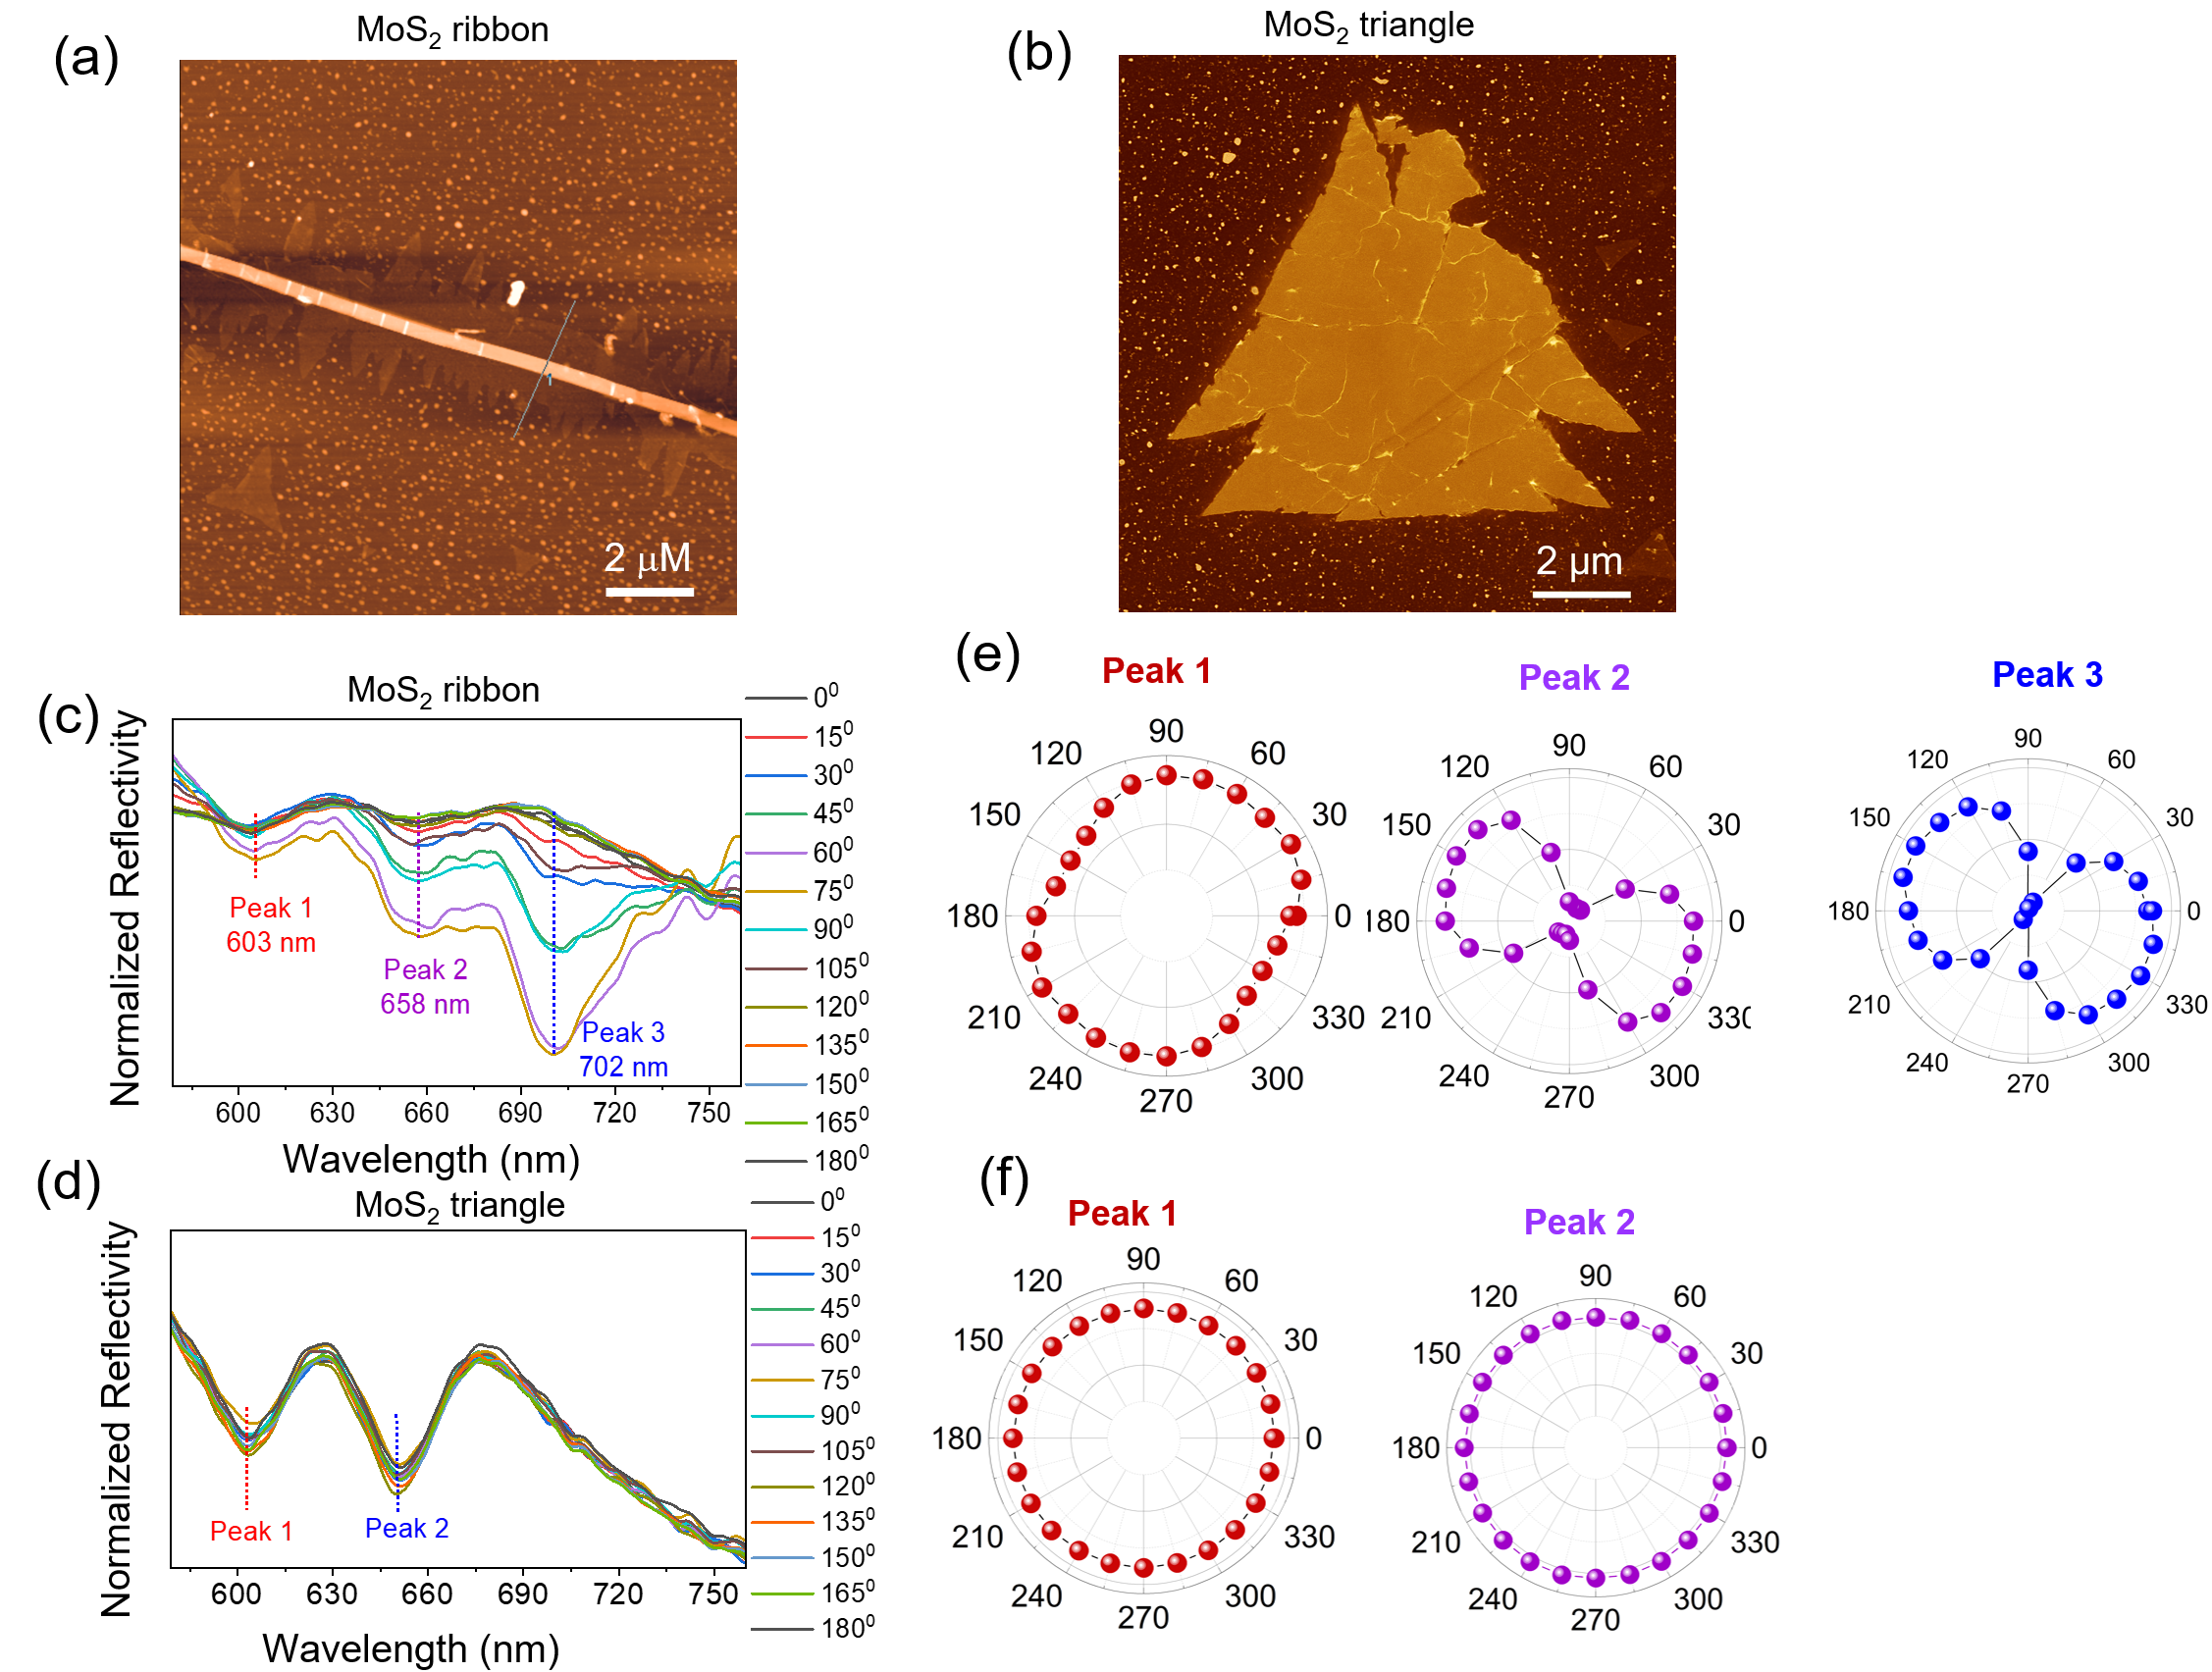
\includegraphics[width=1.0\linewidth]{Figures/Figure_4.png}
    \caption{\textbf{Polarization-resolved reflectance spectra of \ch{MoS2} nanoribbon and triangular flake.} (a) AFM image of a \ch{MoS2} nanoribbon on a \ch{SiO2/Si} substrate. (a,b) Atomic force microscopy (AFM) images of a \ch{MoS2} nanoribbon (height $\sim$20 nm) and a triangular \ch{MoS2} flake, respectively (scale bars: 2 µm). Normalized reflectance spectra of the \ch{MoS2} nanoribbon measured at different polarization angles, showing three prominent spectral features labelled as Peak 1, Peak 2, and Peak 3. 
(d) Normalized reflectance spectra of the triangular \ch{MoS2} flake under polarization rotation, exhibiting two main spectral features (Peak 1 and Peak 2).  Normalized reflection spectra of the \ch{MoS2} nanoribbon (c) and triangular monolayer (d) measured at different polarization angles. (e) Polar plots of the polarization-dependent intensity for Peaks 1–3 of the nanoribbon, revealing pronounced anisotropic optical response. 
(f) Corresponding polar plots for the triangular flake (Peaks 1 and 2), showing nearly isotropic behavior compared to the nanoribbon.}
    \label{fig:polar_reflect}
\end{figure}

To further quantify the observed anisotropic response, we performed identical measurements on a monolayer 
triangular MoS$_2$ ~Figure~\ref{fig:polar_reflect}b. As expected for a 2H phase monolayer with hexagonal 
symmetry, the differential reflectance spectra (~Figure~\ref{fig:polar_reflect}d) reveal only the A and B excitons, both of which show negligible polarization dependence (~Figure~\ref{fig:polar_reflect}f). The isotropic behavior of the monolayer, together with the strongly anisotropic response of the nanoribbon, demonstrates that symmetry breaking and light–matter interactions become profoundly altered when transitioning from 2D to  geometries. The observed anisotropies are further supported by complementary polarization resolved differential reflectance experiments on multiple nanoribbons of different widths and thicknesses, presented in Supplementary Information Figure~S\ref{fig:si_5_width_dependent_anisotropy}, Figure~S\ref{fig:si_6_width_dependent_anisotropy_wider} and Figure~S\ref{fig:si_5_width_dependent_anisotropy_narrower}.
An intermediate width (width $\sim$ 600 nm, thickness $\sim$ 30.2 nm; 

Figure~\ref{fig:si_5_width_dependent_anisotropy} with the excitonic resonances with two well resolved resonances at 603 nm, 672 nm, nearly isotropic and FP mode at several 760 nm shows markedly weaker anisotropy, exhibits modest angular dependence, consistent with a partially confined cavity mode, now a second ribbon of wider ribbon width ($\sim$ 500 nm; $\sim$1\,$\mu$m Figure~S\ref{fig:si_6_width_dependent_anisotropy_wider}) shows only two well resolved resonances at 603 nm, 672 nm, and FP mode
is completely suppressed. This behavior confirms that lateral optical confinement is essential for sustaining strong excitonic anisotropy. Finally, a narrower ribbon (width $\sim$ 300 nm, thickness $\sim$ 22.5 nm; Figure~\ref{fig:si_5_width_dependent_anisotropy_narrower}) supports three well-resolved resonances at 603 nm, 652 nm, and 681 nm, all displaying strong twofold angular modulation. In this highly confined case, the FP-assisted mode shifts toward the excitonic resonances, and all three spectral features exhibit enhanced anisotropy, further illustrating the decisive role of ribbon width in shaping exciton–photon coupling. The polarization-dependent differential reflectance measurements establish 
that MoS$_2$ nanoribbons support a highly orientation-sensitive excitonic response, 
especially in the B exciton and cavity-enhanced FP modes. These optical signatures, which are entirely absent in monolayer MoS$_2$, highlight the emergence of strong optical anisotropy driven by lateral confinement, modified stacking order, and  geometry. These results provide compelling evidence of symmetry breaking in the MoS$_2$ nanoribbons.

%merged discussion Second-harmonic generation (SHG) serves as a highly sensitive probe of broken inversion symmetry and stacking order in layered TMDs. While SHG has been extensively studied in 2D \ch{MoS2} crystals, reports on SHG from  \ch{MoS2} nanoribbons remain scarce. To elucidate the nonlinear optical response of our nanoribbons, we performed SHG imaging using a 785 nm pulsed excitation source, collecting the generated second-harmonic signal in a backscattering configuration. Representative SHG maps of the nanoribbons are shown in Figure~\ref{fig:SHG}.The nanoribbons display uniformly strong SHG emission across their entire length, as seen in Figure~\ref{fig:SHG}a. Notably, the intensity remains nearly constant even when the nanoribbons are rotated with respect to the incident polarization (Figures~\ref{fig:SHG}b–e). This behavior is markedly different from that of conventional 2H-phase \ch{MoS2} monolayers, where SHG intensity varies strongly with both layer number and crystal orientation due to the presence or absence of inversion symmetry.\cite{LightSciAppl2016} In contrast, 3R-phase \ch{MoS2}, which lacks inversion symmetry regardless of thickness, exhibits robust and orientation-independent SHG emission—consistent with our observations.STEM characterization confirms that the nanoribbons predominantly adopt the 3R stacking polytype. In this configuration, each monolayer is laterally shifted relative to the one below, preserving a non-centrosymmetric structure across multiple layers. The persistence of strong SHG intensity for all rotational orientations therefore indicates a uniform crystal phase and the absence of mixed stacking domains within the nanoribbons. The uniformity of the SHG maps also suggests high crystallinity and minimal structural disorder, as defect-induced symmetry breaking typically produces spatially fluctuating SHG signals.Taken together, the nonlinear optical measurements corroborate the structural assessments and provide compelling evidence that the \ch{MoS2} nanoribbons exhibit 3R stacking with consistently broken inversion symmetry. This stacking configuration further supports the anisotropic Raman and differential reflectance results, highlighting the distinct symmetry environment of the nanoribbons and reinforcing their potential for polarization-resolved photonics and nonlinear optical devices.Figure~\ref{fig:SHG} presents the polarization-dependent SHG response of the MoS$_2$ nanoribbon. The optical microscope image in Figure~\ref{fig:SHG}a shows a well-defined MoS$_2$ nanoribbon surrounded by a monolayer flake. Figure~\ref{fig:SHG}(c-k) shows the corresponding SHG maps acquired under different incident linear polarizations. As the pump polarization is rotated from $+40^\circ$ to $-40^\circ$, the SHG emission from the star-shaped flake varies periodically, producing alternating bright and dim features that reflect the underlying lattice symmetry. This behavior is consistent with the expected angular dependence $I_{\mathrm{SHG}} = I_{0}\cos^{2}(3\theta)$ for materials exhibiting broken inversion symmetry and D$_{3h}$-type rotational characteristics. When the excitation polarization aligns with the armchair crystallographic direction (e.g., $0^\circ$ and $-10^\circ$), the SHG intensity reaches its maximum due to efficient coupling between the pump field and the nonlinear polarization of the ABC-stacked 3R lattice. In contrast, orientations near $\pm 30$--$40^\circ$ correspond to mirror-plane directions of the crystal, resulting in suppressed SHG emission in agreement with the symmetry-forbidden directions predicted for 3R MoS$_2$. The SHG polar plot in panel (c) reveals a distinct six-fold rotational symmetry originating from the \ch{MoS2} monolayer edges. The symmetry is preserved in the thin active region of the nanoribbon, indicating that the nanoribbon inherits the intrinsic crystalline orientation of the parent monolayer. Furthermore, the observed SHG intensity modulation reflects the expected thickness dependence characteristic of non-centrosymmetric \ch{MoS2}, demonstrating that the nonlinear optical response remains highly sensitive to local structural variations within the ribbon. The polarization-dependent SHG response of the MoS$_2$ ribbons provides further key insights into their stacking order, thickness, and crystallographic orientation. The bulk ribbons exhibit a clear polarization dependence characteristic of non-centrosymmetric stacking, consistent with either 2H or 3R MoS$_2$. AFM measurements show that the thickness of the ribbons corresponds closely to the reported band I thickness regime for 3R-MoS$_2$, where significantly enhanced SHG intensity is expected \cite{Shi2017}. This correlation between the measured thickness and predicted SHG activity strongly suggests that the ribbons crystallize in the 3R stacking phase rather than the centrosymmetric 2H phase.




%\section{Electrical measurement}
%Polarization-dependent electrical measurement To study the gate-dependent anisotropic electrical properties, the \ch{MoS2} nanorod devices were fabricated on a 300 nm thick Si/SiO2 layer with the underlying conducting Si substrate as a back gate. Figure … shows a typical \ch{MoS2} nanorod with a channel length of ... $\mu$m between Cr/Au contacts. The width is about 100 nm, and the height is about 32 nm from AFM measurements, a nanoribbon shape consistent with \ch{MoS2} nanorod. Figure .. shows linear I-V behavior with a conductivity .. S/cm. Measurements conducted over several devices show that the conductivity of \ch{MoS2} nanorod with growth direction is in the range of ... S/cm. Gate voltage-dependent transport measurements were also carried out at room temperature. Figure … shows I-V curves at different gate voltages (Vg). Figure … shows the I-Vg curve at fixed Vsd at 5V. When Vg is made increasingly negative (positive), the conductance decreases (increases). Special photocurrent measurements were performed with two different polarization directions to understand the photo-current generation from 1D \ch{MoS2} nanoribbons. Again, the polarization-dependent current measurement from \ch{MoS2} nanoribbons displayed a significant variation in parallel and cross-polarization excitation. Figure 7a shows the photocurrent measures as a function of polarization at VDS= from 0V to 5V under parallel and cross-polarization.The polarization-sensitive photocurrent measurement by scanning the linearly-polarized light over the device. The anisotropic photocurrent is observed to be maximum when the light polarization is perpendicular to the crystal axis. The photocurrent anisotropy ratio is calculated as Y= (Ipmax-Ipmin)/(Ipmax+Ipmin)~0.5, which is quite significant.

To systematically investigate anisotropic charge transport and polarization dependent photocurrent generation, two terminal MoS$_2$ nanoribbon devices were fabricated on Si/SiO$_2$ substrates with a 300~nm thermally grown SiO$_2$ dielectric layer. A schematic illustration of the device architecture is shown in ~Figure~\ref{fig:MoS2_polarization_electrical}a, where a single MoS$_2$ nanoribbon bridges two metallic electrodes and is illuminated with a linearly polarized 532~nm laser. Electrical contacts were defined using Cr/Au (5/50~nm) electrodes, where Cr serves as an adhesion layer, and Au provides low-resistance electrical conduction. The electrodes were patterned using standard UV photolithography, followed by metal deposition and lift off, yielding well aligned, reproducible devices. Atomic force microscopy (Figure~\ref{fig:synthesis_schematic}c) confirms a nanoribbon thickness of approximately 23~nm, corresponding to a multilayer structure.

\begin{figure}[H]
\centering
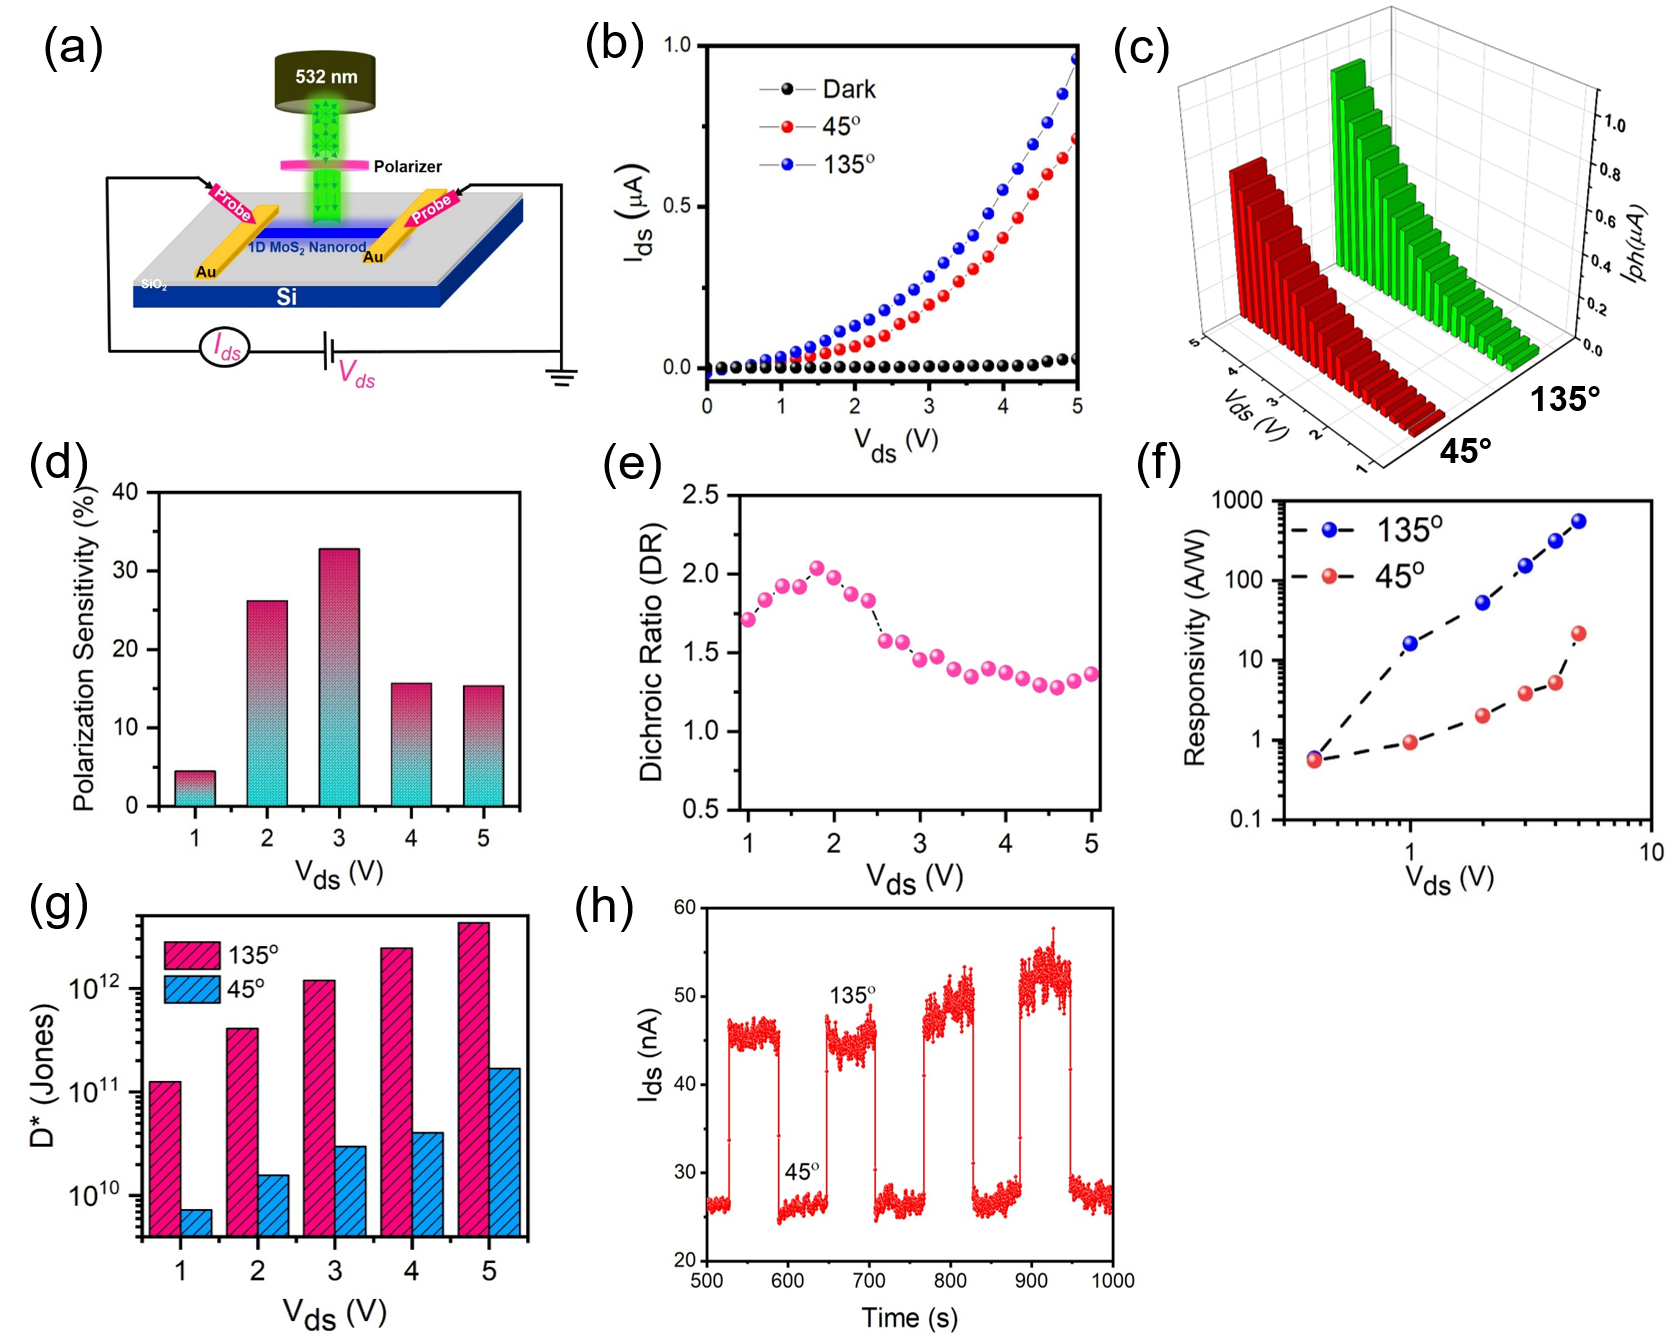
\includegraphics[width=0.95\linewidth]{Figures/Figure_6_new_updated2.png}
\caption{\textbf{Polarization-dependent photodetection in a MoS$_2$ nanoribbon device.}
(a) Schematic illustration of the MoS$_2$ nanoribbon photodetector fabricated on a SiO$_2$/Si substrate under polarized 532~nm illumination.
(b) Output characteristics ($I_{ds}$–$V_{ds}$) measured in the dark and under polarized illumination at 45$^\circ$ and 135$^\circ$, showing pronounced polarization-dependent photocurrent.
(c) Three-dimensional map of drain current as a function of bias voltage and polarization angle, highlighting strong anisotropic photoresponse.
(d) Extracted polarization sensitivity as a function of bias voltage.
(e) Dichroic ratio versus bias, confirming robust polarization selectivity with enhanced response at 135$^\circ$.
(f) Responsivity as a function of bias voltage for different polarization states, reaching 551~A\, W$^{-1}$ at 135$^\circ$.
(g) Specific detectivity as a function of bias voltage.
(h) Time-resolved photocurrent showing stable polarization switching.}
\label{fig:MoS2_polarization_electrical}
\end{figure}

The current–voltage ($I_{ds}$–$V_{ds}$) characteristics measured under dark and polarized illumination at 45$^\circ$ and 135$^\circ$ are shown in ~Figure~\ref{fig:MoS2_polarization_electrical}b. Illumination produces a substantial increase in current compared to the dark condition, confirming photoconductive behaviour. Notably, the photocurrent magnitude depends strongly on polarization angle, with significantly higher current observed at 135$^\circ$. This pronounced anisotropy indicates that both optical absorption and carrier transport are directionally dependent within the nanoribbon. The enhanced photocurrent at 135$^\circ$ arises from improved coupling between the incident electric field and the nanoribbon's preferred structural axis, thereby enabling more efficient photocarrier generation. In contrast, misalignment at 45$^\circ$ reduces light–matter interaction and photocurrent generation. As the bias increases, the applied electric field promotes carrier separation and suppresses recombination, further amplifying the intrinsic anisotropic photoresponse.
The polarization dependence of the photocurrent is summarized in the three dimensional map shown in ~Figure~\ref{fig:MoS2_polarization_electrical}c, where the photocurrent ($I_{ph} = I_{light} - I_{dark}$) is plotted as a function of drain bias and polarization angle. The consistently higher photocurrent at 135$^\circ$ confirms strong intrinsic anisotropy governed by the  geometry of the nanoribbon. The polarization sensitivity (PS), defined as

\begin{equation}
PS = \frac{I_{\max} - I_{\min}}{I_{\max} + I_{\min}},
\end{equation}

\noindent
where $I_{\max}$ and $I_{\min}$ correspond to the photocurrent at 135$^\circ$ and 45$^\circ$, respectively, is plotted in ~Figure~\ref{fig:MoS2_polarization_electrical}d. The PS increases with increasing bias and reaches a maximum at 3~V, reflecting enhanced carrier separation and drift transport. At higher bias, the PS exhibits slight saturation, likely due to increased dark current contribution, carrier scattering, and partial screening of polarization-dependent absorption.
The dichroic ratio (DR), which quantifies polarization selectivity, is defined as

\begin{equation}
DR = \frac{I_{\max}}{I_{\min}}.
\end{equation}

\noindent
As shown in ~Figure~\ref{fig:MoS2_polarization_electrical}e, the DR remains consistently greater than unity across the entire bias range, demonstrating robust polarization discrimination in the MoS$_2$ nanoribbons.
The polarization resolved responsivity ($R_{\lambda}$) and specific detectivity ($D^*$) were further evaluated and are presented in ~Figure~\ref{fig:MoS2_polarization_electrical}f and ~Figure~\ref{fig:MoS2_polarization_electrical}g. These parameters were calculated using

\begin{equation}
R_{\lambda} = \frac{I_{ph}}{P_{\lambda} S}
\end{equation}

\begin{equation}
D^* = \frac{R_{\lambda} \sqrt{S}}{\sqrt{2 e I_{dark}}},
\end{equation}

\noindent
where $I_{ph}$ is the photocurrent, $P_{\lambda}$ is the incident optical power, $S$ is the illuminated area, and $e$ is the elementary charge. The responsivity reaches 551~A\,W$^{-1}$ and detectivity reaches $4.3 \times 10^{12}$ Jones at 135$^\circ$, which are nearly an order of magnitude higher than the values obtained at 45$^\circ$ (22~A\,W$^{-1}$ and $1.7 \times 10^{11}$ Jones). This substantial enhancement confirms the highly anisotropic photodetection capability of the nanoribbons.

The dynamic photoresponse under alternating polarization states is shown in ~Figure~\ref{fig:MoS2_polarization_electrical}h. The photocurrent exhibits stable, repeatable switching between high and low current levels corresponding to polarization angles of 135$^\circ$ and 45$^\circ$, respectively. The reproducibility and stability of the switching behavior confirm reliable polarization-sensitive photodetection. The observed anisotropic photoresponse is consistent with the vibrational and optical anisotropy revealed by Raman spectroscopy and differential reflectance measurements. These results demonstrate that MoS$_2$ nanoribbons exhibit direction dependent carrier transport and photogeneration efficiency arising from their  morphology, 3R stacking configuration, and symmetry broken electronic structure. This pronounced anisotropy highlights the potential of MoS$_2$ nanoribbons for applications in polarization-sensitive photodetectors, orientation-selective phototransistors, and advanced anisotropic optoelectronic devices.



\section{Conclusions}

In conclusion, we have demonstrated growth of a new  form of multilayer MoS$_2$ in which geometric confinement and noncentrosymmetric stacking generate pronounced optical and electronic anisotropy. The nanoribbons, synthesized via a liquid-mediated sulfurization pathway, exhibit structural characteristics fundamentally distinct from conventional 2H  MoS$_2$, most notably a predominant 3R stacking order that preserves broken inversion symmetry across multiple layers. This symmetry breaking manifests consistently across vibrational, optical, and electrical probes, establishing the nanoribbons as intrinsically anisotropic quantum structures.
Polarization-resolved Raman spectroscopy reveals a strong twofold modulation of both the $A_{1g}$ and $E^1_{2g}$ modes, directly confirming reduced in-plane symmetry and anisotropic electron-phonon coupling. Complementary differential reflectance measurements show polarization-dependent excitonic absorption and cavity-enhanced optical resonances, demonstrating that lateral confinement fundamentally modifies exciton-photon interactions. These linear optical signatures are corroborated by pronounced, orientation-dependent second-harmonic generation, providing direct evidence of persistent inversion-symmetry breaking in multilayer nanoribbons. These symmetry lowered electronic states translate into strongly anisotropic optoelectronic functionality. Polarization-dependent phototransport measurements reveal highly directional photocurrent generation, with responsivity exceeding 551~A~W$^{-1}$ and detectivity reaching $4.3 \times 10^{12}$~Jones, together with stable and reversible polarization switching. The observed anisotropy in photocurrent and excitonic absorption demonstrates that symmetry breaking governs both photocarrier generation and transport, enabling efficient directional charge separation. These results establish  MoS$_2$ nanoribbons as a fundamentally distinct symmetry-engineered platform in which geometric confinement and stacking order define light-matter interactions. Beyond revealing new physics associated with reduced dimensionality, this work provides a scalable route to engineer intrinsic anisotropy and nonlinear optical functionality in layered semiconductors. Such symmetry broken nanoribbons offer significant potential for next generation polarization selective photodetectors, nonlinear photonic devices, and quantum optoelectronic systems in which optical response can be controlled through geometry and crystallographic design.


%%%%%%%%%%%%%%%%%%%%%
% METHODS %
%%%%%%%%%%%%%%%%%%%%%

\section{MATERIALS AND METHODS}
\subsection{Materials synthesis}
\subsubsection{Growth of precursor epitaxial MoO\textsubscript{2} films by PLD}

The precursor oxides were grown by laser ablation of a one-inch MoO\textsubscript{3} target (99.95 percent purity, from Testbourne Ltd.) in Ar at a pressure of 0.1 mbar. The target was ablated using a 248 nm KrF excimer laser operating at 1 Hz. The target-to-substrate distance was ~7 cm. Before deposition, the vacuum chamber was pumped down to a base pressure of ~$6\times 10^{-7}$ mbar, and the target was preablated using 60 laser pulses. All experiments maintained the laser fluence on the target at ~ 2 J/cm\textsuperscript{2}. The films were grown on (0001) Al\textsubscript{3}O\textsubscript{3} substrates at 700\textsuperscript{o}C using a number of laser shots ranging from 5 to 20. Further details of the PLD process are provided elsewhere \cite{WOS:000623061800072}.

\subsubsection{Deposition of the NaF layer}
The 20 nm-thick NaF layer was deposited on top of the oxide precursors by thermal evaporation of NaF powder (purity 99.9, Sigma Aldrich) in high vacuum at a pressure of ~$6\times 10^{-6}$ mbar. The depositions were done in an evaporation chamber from Univex 250 Oerlikon. The thickness of the NaF layers was estimated using an evaporation rate of 0.3\AA/s.

\subsubsection{Synthesis of the \ch{MoS2} nanostructures}  
The high-temperature growth of \ch{MoS2} was carried out in a compact furnace, type OTF-1200X-4-NW-UL, from MTI Corporation. Firstly, the precursor films were placed on a ceramic plate and loaded into the middle of the 4-inch quartz tube. A narrow alumina ceramic boat containing 1.5 g of sulfur flakes (99.99 percent purity, from Sigma Aldrich) was placed outside the central heating zone of the furnace and heated independently using an external heater. The distance between the ceramic boat and the samples was 28 cm. Before sulfurization, the system was pumped down to  $1.6\times 10^{-3}$  mbar and sequentially flushed five times by pressuring the tube to 650 mbar with Ar-5\% H\textsubscript{2} mixture ($99.9995$ \% purity) to remove residual gases. The tube furnace was heated at 25\textsuperscript{o}C per min to 800\textsuperscript{o}C, and the sulfurization process was carried out at 800\textsuperscript{o}C for 10 min. When the furnace temperature reached 800 \textsuperscript{o}C, the external heating zone containing the sulfur boat reached a temperature of 230 \textsuperscript{o}C. The system was cooled at a rate of 20 \textsuperscript{o}C/min to 600\textsuperscript{o}C and then allowed to cool naturally to room temperature. A constant Ar-5\% H\textsubscript{2} gas flow of 100 sccm was maintained throughout the process.

\subsubsection{Materials characterisation}
Raman and PL spectra were collected using a home-built Raman confocal spectroscopy setup using a 532 nm excitation laser. The spectrometer is a Spectra Pro HRS-750 scanning monochromator from Princeton Instruments, equipped with three gratings at 300, 1200, and 1800 gr/mm, and a cryogenically cooled, ultra-low-noise Pylon CCD camera, type PyLoN:100BR. The wavelength calibration was performed using an Ar-Ne light source mounted directly at the spectrometer's entrance slit. The spectrometer resolution is 1 cm\textsuperscript{-1}.
 Raman and PL spectra were collected using 300 gr/mm and 1800 gr/mm gratings, respectively, and the laser power was kept below 1 mW to prevent overheating of the sample.
 
The second-harmonic generation (SHG) data were acquired on a confocal system using an ultrashort-pulse laser at 785 nm (pulse duration of 2 ps, repetition rate of 80 MHz, 20 mW). The specimens were illuminated through an objective lens (100X, numerical aperture (N.A.) 0.95), resulting in a diffraction-limited spot size with a full width at half maximum of.. nm. A motorized half-wave plate continuously tunes the polarisation of the incident laser. The resulting SHG signal is collected with the same objective and passed through a dichroic mirror. In our experiment, given the relatively small diameter of the  nanoribbons, a change in the laser beam position on the sample may lead to a considerable variation in SHG intensity. Our SHG measurements and signals were collected to ensure accuracy and consistency by fixing the linear analyzer in a particular direction. 

The high-resolution SEM images were acquired using a Zeiss Merlin microscope equipped with an InLens detector. The nanostructures were imaged using low-acceleration voltages (1–2 kV) and short working distances (3-4 mm).

The atomic force microscopy (AFM) images were measured on a Dimension Icon AFM (AFM Icon-PT 2 from Bruker) using  Al-coated Si probe tips (type Tap150Al-G from BudgetSensors). The measurements were carried out in non-contact mode in ambient air. 


\subsubsection{Device fabrication and characterization}
The \ch{MoS2} nanoribbons obtained from two-step growth methods were used to fabricate the electrical devices. Using the above procedure, the as-grown \ch{MoS2} nanoribbons were transferred to the (300 nm) SiO\textsubscript{2}/Si substrate. The patterns on top of the nanoribbons were formed by UV lithography in the clean room, and 5 nm/50nm Cr/Au was deposited for the metal contacts. Keithley instruments were used to perform the electrical measurements. A halogen fiber-optic light source was used to illuminate the sample, and the white light was coupled into a monochromator for photoconductivity measurements. Two-terminal device contacts with source and drain contacts were used, where both current and voltage drop were measured. 

\section{Acknowledgements}
 S.C. acknowledges support from the Independent Research Fund Denmark, Sapere Aude grant (project number 8049-00095B. STEM imaging was conducted as a part of a user project at the Center for Nanophase Materials Sciences, a DOE Office of Science User Facility. R. K. U. would like to acknowledge the Prime Minister Early Career
Research Grant (PM-ECRG) from the Anusandhan National Research Foundation (ANRF),
India, under Grant Code No. ANR-2670-NTC-CNA/25. C.P. and B.M. acknowledge support from the European Research Council (ERC-StG ``TuneTMD", grant no. 101076437) and the Villum Foundation (grant no. VIL53033).

\bibliography{bibliography}

\begin{suppinfo}
\setcounter{figure}{0}
\renewcommand{\thefigure}{S\arabic{figure}}
\newpage
%%%%%%%%%%%%%%%%%%%%%%%%%%%%%%%%%%%%%%%%%%%%%%%%%%%%
%%%%%%%%%%%%% Commented out %%%%%%%%%%%%%%%%%%%%%%%%
%%%%%%%%%%%%%%%%%%%%%%%%%%%%%%%%%%%%%%%%%%%%%%%%%%%%
\iffalse
\begin{figure}%[htb]
    \centering
    \includegraphics[width=1\linewidth]{Figure 1S.jpg}
    \caption{\textbf{Atomic structures of different adatoms in the PLD-grown MoS\textsubscript{2} monolayer}. (a) Experimental STEM images showing a Mo adatom on a Mo site (a-Mo\textsubscript{Mo}) and S adatoms on a Mo site (a-S\textsubscript{Mo}). (b) The line profiles of the corresponding adatoms reveal a higher intensity indeed for the a-Mo\textsubscript{Mo} than for the Mo atoms in the pristine MoS\textsubscript{2} ML.}
    \label{fig:adatoms_exp}
\end{figure}

\begin{figure}
    \centering
    \includegraphics[width=0.9\linewidth]{fig_adMo.png}
    \caption{Comparison of the experimental (a) and simulated (b) STEM images of the \ch{Mo} adatom in \ch{MoS2} as well as their line profiles (c). Yellow triangles highlight the respective adatoms within the \ch{MoS2} structures.}
    \label{fig:Mo_ad}
\end{figure}

\begin{figure}%[htb]
    \centering
  \includegraphics[width=0.6\linewidth]{Figure 3S.jpg}
    \caption{Figure 3S \textbf{Morphology and grain boundary structures of PLD-grown layered MoS\textsubscript{2} films}. (a) Low magnification ADF STEM image of a MoS\textsubscript{2} monolayer showing nanometer-size domains separated by grain boundaries. False-colored images allow clear distinction of individual grains. (b) Low magnification ADF STEM image showing a large area monolayer (1L) with distinct bilayer regions (2L). \textbf(c,d) Magnified views of the regions highlighted by the yellow rectangle showing the grain boundary structures and the second layer growing along the grain boundary.} 
    \label{fig:morphology}
\end{figure}

\begin{figure}%[htb]
    \centering
  %%  \includegraphics[width=1\linewidth]{Figure SI for figure 3.jpg}
    \caption{Figure 3S \textbf{Atomic resolution image of a 2H/1T grain boundary structure with 30\textsuperscript{o} rotation}. (a) ADF STEM image of a grain boundary where the 2H phase (up) and 1T phase (down) are observed. The overlaid triangles in the different grains are rotated by 30\textsuperscript{o} with respect to each other.(b) Fourier transform (FFT) of the image showing two distinct patterns of diffraction spots with 30\textsuperscript{o} rotation. (c) False-colored FFT-filtered image using the first set of diffraction spot highlighted in pink. (d) False-colored FFT-filtered image using the second set of diffraction spots highlighted in blue. } 
    \label{fig:morphology}
\end{figure}

\begin{figure}%[htb]
    \centering
    \includegraphics[width=1\linewidth]{Figure4S.jpg}
    \caption{Figure 4S \textbf{Atomic resolution image of bilayer MoS\textsubscript{2} formed by overlapped of two grains with 17\textsuperscript{o} rotation}. (a) ADF STEM image of moir\'e pattern formed as a result of an overlapped junction.(b) Schematic showing the second .(b) Fourier transform (FFT) of the image showing two distinct patterns of diffraction diffraction spots with 17\textsuperscript{o} rotation. (c) FFT-filtered image using the first set of diffraction spot highlighted in yellow and showing monolayer one (Layer 1). (d) FFT-filtered image using the second set of diffraction spot highlighted in blue showing the monolayer 2 growing on top of Layer 1 with and rotated by  17\textsuperscript{o} rotation with respect to the ther gain. The } 
    \label{fig:morphology}
\end{figure}
\begin{figure}%[htb]
    \centering
    \includegraphics[width=1\linewidth]{Figure 5S.jpg}
    \caption{Figure 4S \textbf{Atomic resolution image of bilayer MoS\textsubscript{2} formed by overlapped of two grains with 17\textsuperscript{o} rotation}. (a) STEM HAADF image of moir\'e pattern formed as a result of an overlapped junction.(b) Schematic showing the second .(b) Fourier transform (FFT) of the image showing two distinct patterns of diffraction spots with 17\textsuperscript{o} rotation. (c) FFT-filtered image using the first set of diffraction spots highlighted in yellow and showing monolayer one (Layer 1). (d) FFT-filtered image using the second set of diffraction spots highlighted in blue showing the monolayer 2 growing on top of Layer 1 with and rotated by  17\textsuperscript{o} rotation with respect to their gain. The }
    \label{fig:morphology}
\end{figure}

\begin{figure}%[htb]
    \centering
    \includegraphics[width=1\linewidth]{Figure 6S.jpg}
    \caption{Figure 4S \textbf{Atomic resolution image of bilayer MoS\textsubscript{2} formed by overlapped of two grains with 17\textsuperscript{o} rotation}. (a) ADF STEM image ofmoir\'e  pattern formed as a result of an overlapped junction.(b) Schematic showing the second .(b) Fourier transform (FFT) of the image showing two distinct patterns of diffraction spots with 17\textsuperscript{o} rotation. (c) FFT-filtered image using the first set of diffraction spot highlighted in yellow and showing monolayer one (Layer 1). (d) FFT-filtered image using the second set of diffraction spot highlighted in blue showing the monolayer 2 growing on top of Layer 1 with and rotated by  17\textsuperscript{o} rotation with respect to the ther gain. The } 
        \label{fig:morphology}
\end{figure}
\begin{figure}%[htb]
    \centering
    \includegraphics[width=1\linewidth]{Figure 7S.jpg}
    \caption{Figure 4S AB or AA' phase transition induced by electron beam at room temperature. No final
    } 
        \label{fig:morphology}
\end{figure}

The following files are available free of charge.
\begin{itemize}
 
\end{itemize}
\fi 
%%%%%%%%%%%%%%%%%%%%%%%%%%%%%%%%%%%%%%%%%%%%%%%%%%%%
%%%%%%%%%%%%% Commented out %%%%%%%%%%%%%%%%%%%%%%%%
%%%%%%%%%%%%%%%%%%%%%%%%%%%%%%%%%%%%%%%%%%%%%%%%%%%%

  \item \texttt{SI.pdf}: Supplementary Figures S1-S7.
  


\setcounter{figure}{0}
\renewcommand{\thefigure}{S\arabic{figure}}
\begin{itemize}
\section*{Supplementary Note 1}
\textbf{Measurement schematic:}

\begin{figure}
    \centering
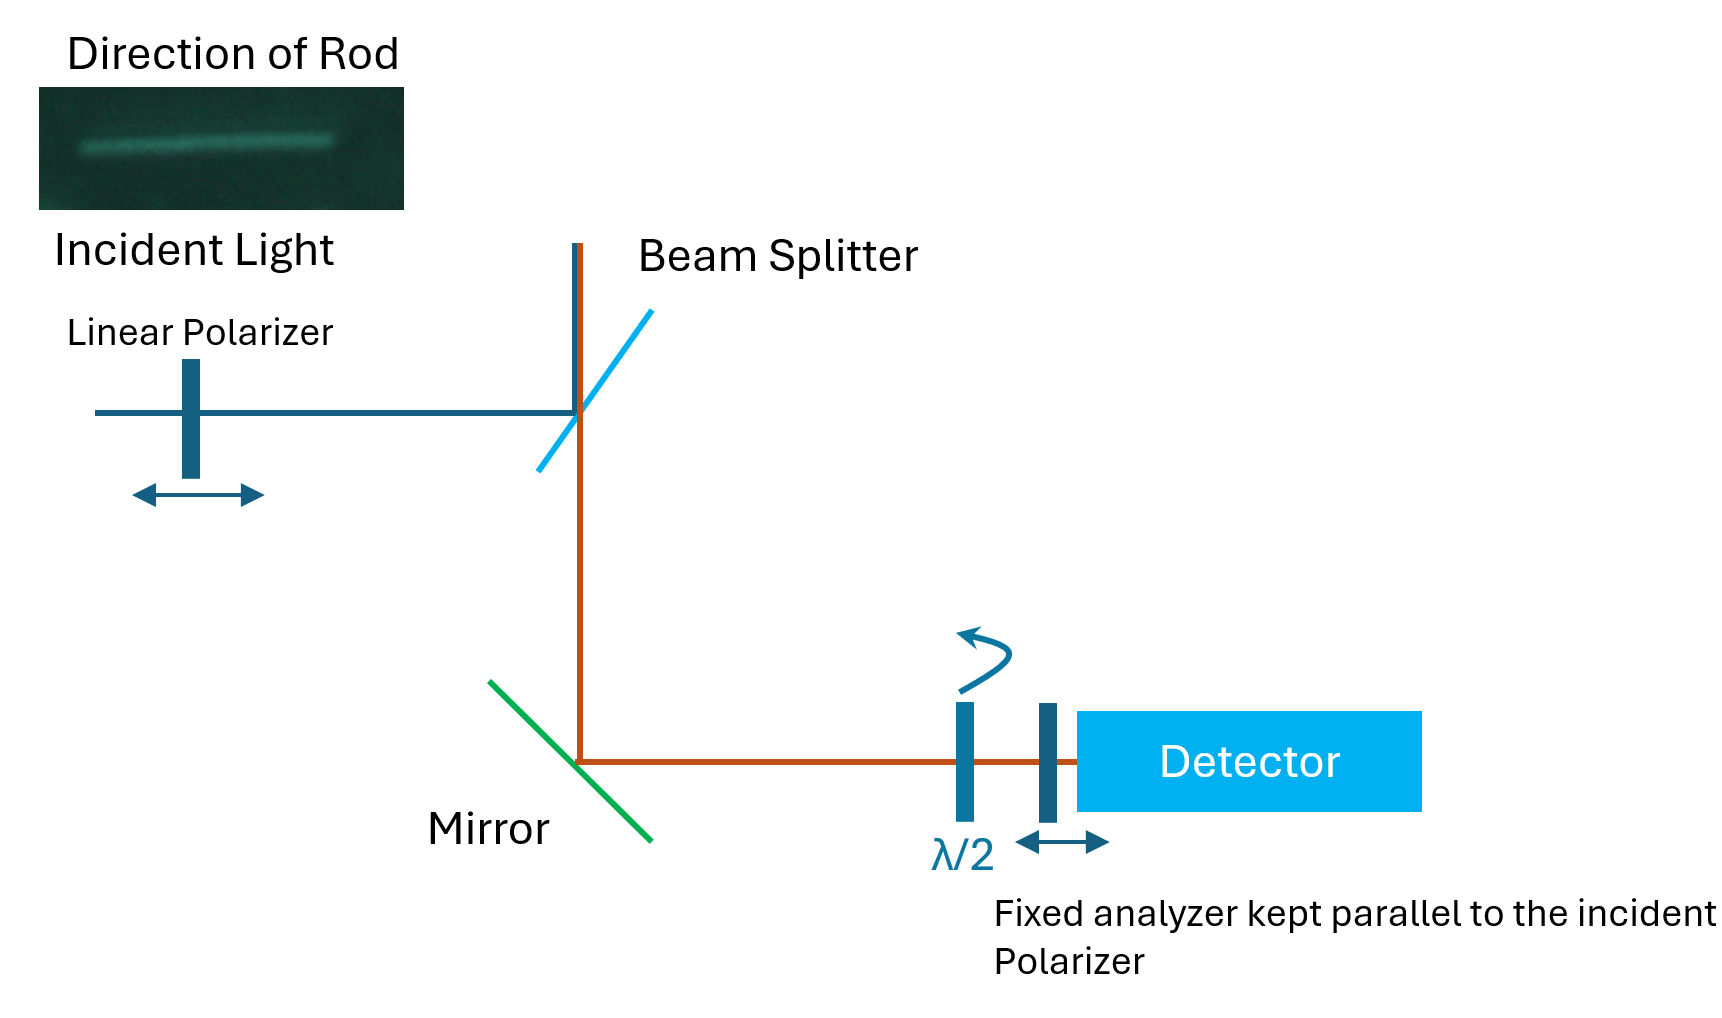
\includegraphics[width=0.9\linewidth]{Figures SI/Figure S1_setup Raman Pol.png}
\caption{\textbf{Schematic of the polarization resolved measurement setup used for the measurements.} Experimental Linearly polarized incident light is directed onto the MoS$_2$ nanoribbon through a beam splitter, with the polarization axis defined relative
to the ribbon orientation. The reflected beam is routed to the detector after passing
through a rotatable $\lambda/2$ wave plate and a fixed analyzer kept parallel to the
incident polarizer. During the measurement, the sample is rotated while the detection
polarization remains fixed, enabling the extraction of angle-dependent optical
responses.}
    \label{fig:schematic sample rotation}
\end{figure}

Figure~\ref{fig:schematic sample rotation} illustrates the optical configuration used to measure the polarization dependent response of the MoS$_2$. A linearly polarized beam is generated using a polarizer, which defines the incident polarization direction. The MoS$_2$ nanoribbon sample is mounted on a stage, and Raman spectra are recorded between a rotating  polarizer  and fixed analyzer. The rotation is performed around the horizontal $x$-axis of the Raman microscope sample stage, such that the reported angles correspond directly to the rotation angle of the nanoribbon relative to the horizontal axis. The incident beam reaches the sample through a beam splitter, and the reflected signal is directed to the detection path via a mirror. A half wave plate ($\lambda/2$) is placed before the detector to maintain a constant detection polarization condition. The analyzer is kept parallel to the incident polarizer to ensure that only the modulation induced by the sample is recorded. In this configuration, the polarization state of the incident light physically rotated from $0^\circ$ to $360^\circ$. This approach enables direct probing of the intrinsic optical anisotropy of the nanoribbons, since any variation in the measured intensity arises solely from the orientation-dependent light matter interaction.

\section*{Supplementary Note 2}
\textbf{Anisotropic Raman response of \ch{MoS2} nanoribbons:} 

To really nail down the anisotropic vibrational behavior in these  MoS$_2$ nanoribbons, we ran angle resolved Raman spectroscopy. We rotate  the polarization state of the incident light physically rotated from $0^\circ$ to detection light polarizations fixed. In Figure~\ref{fig:si_Mo_ribbon-Sample rotation}a and b, the Raman spectra at different angles and their changes how the $E^1_{2g}$ (in-plane) and $A_{1g}$ (out-of-plane) modes change as we rotate. Both modes show clear, strong angular modulation, which tells us the vibrations depend a lot on how the nanoribbon's oriented. Now, if you look at the polar plots in Figure~\ref{fig:si_Mo_ribbon-Sample rotation}c and d, the $A_{1g}$ mode stands out with sharp twofold symmetry peaks and valleys that line up nicely. That means out-of-plane vibrations interact with the optical field in a way that depends on the ribbon's axis. The in-plane $E^1_{2g}$ mode isn't as dramatic, but you still see a definite anisotropy, which fits with changes in the in-plane force constants probably due to the lattice distortion or symmetry breaking because of the nanoribbon's  shape.
This is totally different from what you get in regular monolayer or bulk MoS$_2$, where the Raman response doesn't change, because of its hexagonal symmetry. But here, the --1D structure brings in preferred bonding directions, strain, and local changes in dielectric screening of which throw off the usual Raman tensor and make the scattering intensity depend on angle. These findings supports the argument made in the main text as by shrinking MoS$_2$ down from 2D to  makes its vibrational and optical properties a lot more direction dependent.


\begin{figure}
    \centering
    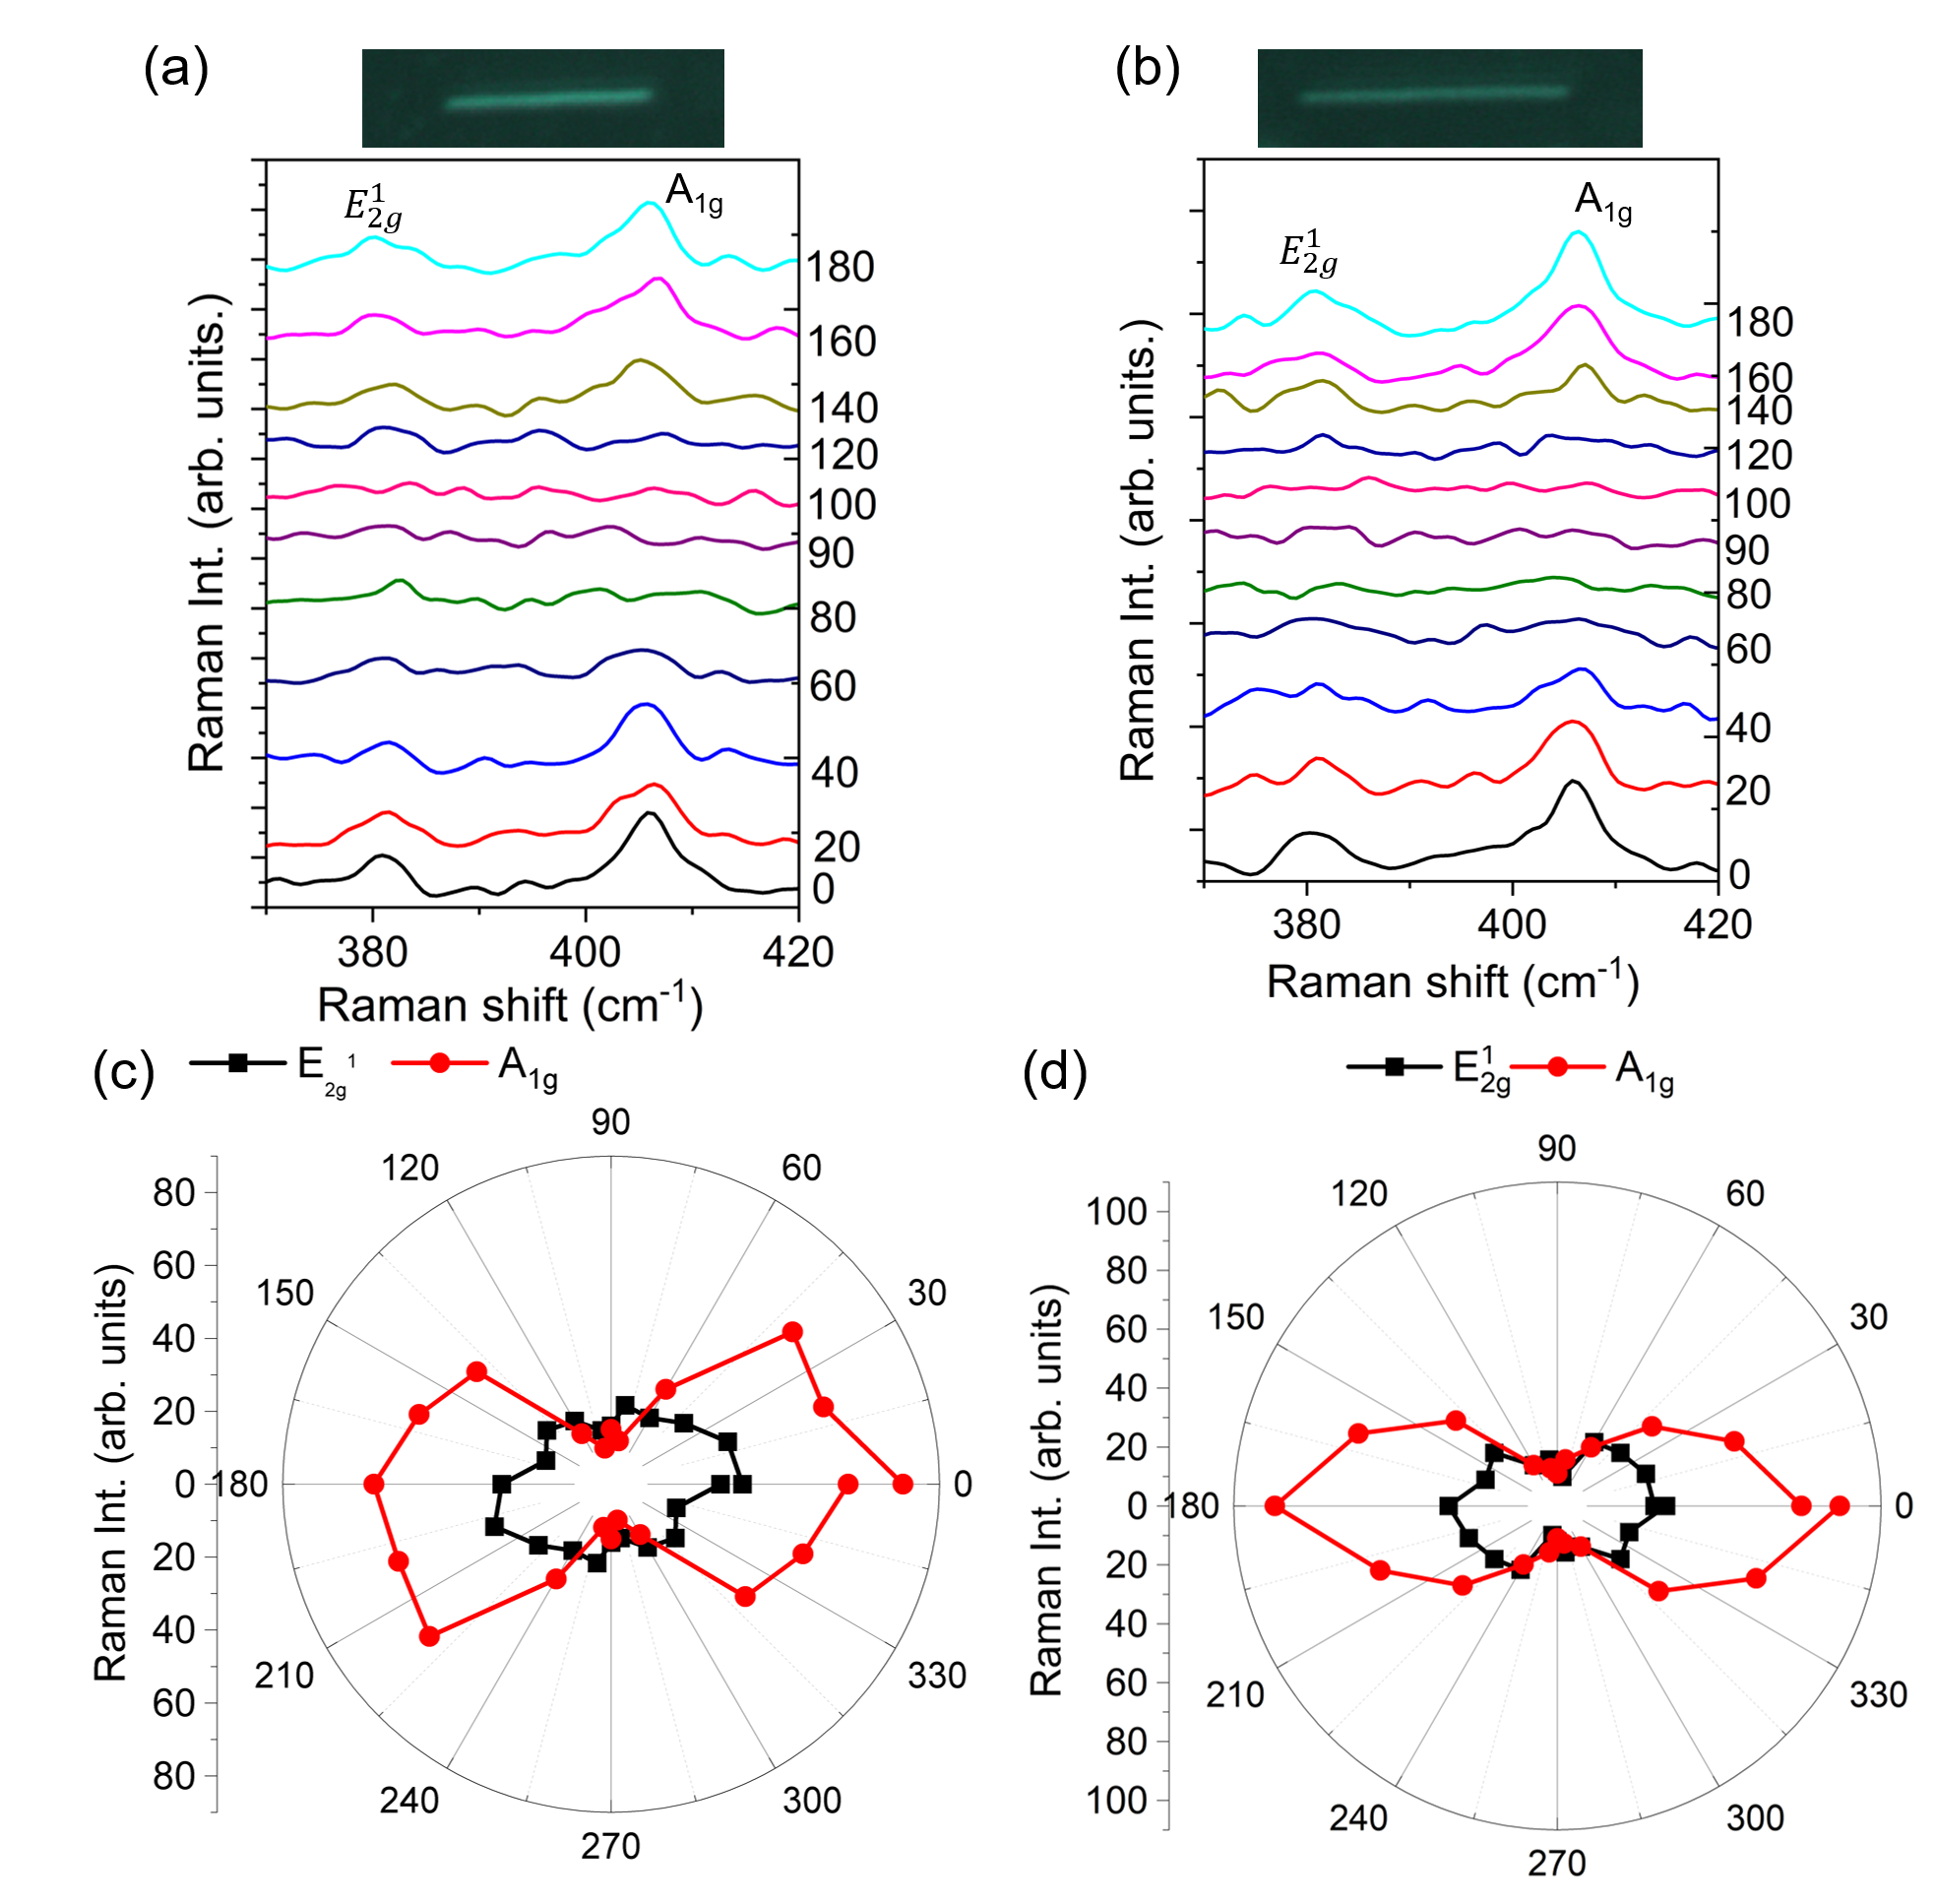
\includegraphics[width=0.9\linewidth]{Figures SI/Figure S2_polRaman rods.png}
    \caption{\textbf{Anisotropic Raman response of MoS\textsubscript{2} nanoribbons.}. (a,b) Raman spectra of a MoS\textsubscript{2} nanoribbon recorded at different sample rotation angles, of two different nanoribbons showing the evolution of the $E_{2g}^{1}$ and $A_{1g}$ modes. 
(c,d) Polar plots of the integrated intensities of the two Raman modes, revealing pronounced angular anisotropy arising from the  geometry of the nanoribbon.}
    \label{fig:si_Mo_ribbon-Sample rotation}
\end{figure}

\section{Supplementary Note 3} 
\textbf{Isotropic Raman response of triangular \texorpdfstring{MoS$_2$}:} To quantify further the anisotropic Raman behavior in the  MoS$_2$ nanoribbons, we did anisotropic Raman measurements on a monolayer triangular MoS$_2$ flake. Since monolayer MoS$_2$ has a 2H crystal structure with sixfold symmetry in the plane, you expect it to show a totally different angular Raman response than the low symmetry nanoribbons.
Figure~\ref{fig:si_2D_Triangular MoS2}a,  shows the angle resolved Raman spectra we got as we rotated from $0^\circ$ to $360^\circ$. Two main phonon modes the in plane $E^1_{2g}$ and the out-of-plane $A_{1g}$ and their polarization behaviors, shown in the polar plots in Figure~\ref{fig:si_2D_Triangular MoS2}b, show the sort of anisotropy you’d expect from selection rules in monolayer MoS$_2$.
The $E^1_{2g}$ mode pretty much keeps the same intensity as you rotate it, which fits with its in plane vibrational character and the hexagonal symmetry of the crystal. The $A_{1g}$ mode, on the other hand, gives you a strong two-lobe pattern in the polar plot this comes from its out-of-plane vibrations and its well known sensitivity to the angle between the incident polarization and the crystal axes. Seeing this weak angular change for $E^1_{2g}$, strong for $A_{1g}$ is classic monolayer 2H-MoS$_2$. What really jumps out is how isotropic the $E^1_{2g}$ phonon is in the monolayer, compared to the strong Raman anisotropy we saw in the nanoribbons. That contrast makes it clear that the observed anisotropy in the nanoribbons doesn’t come from MoS$_2$’s basic crystal symmetry innstead, it’s from symmetry breaking from lateral confinement, edge effects, and the  shape.

\begin{figure}%[t]
    \centering
    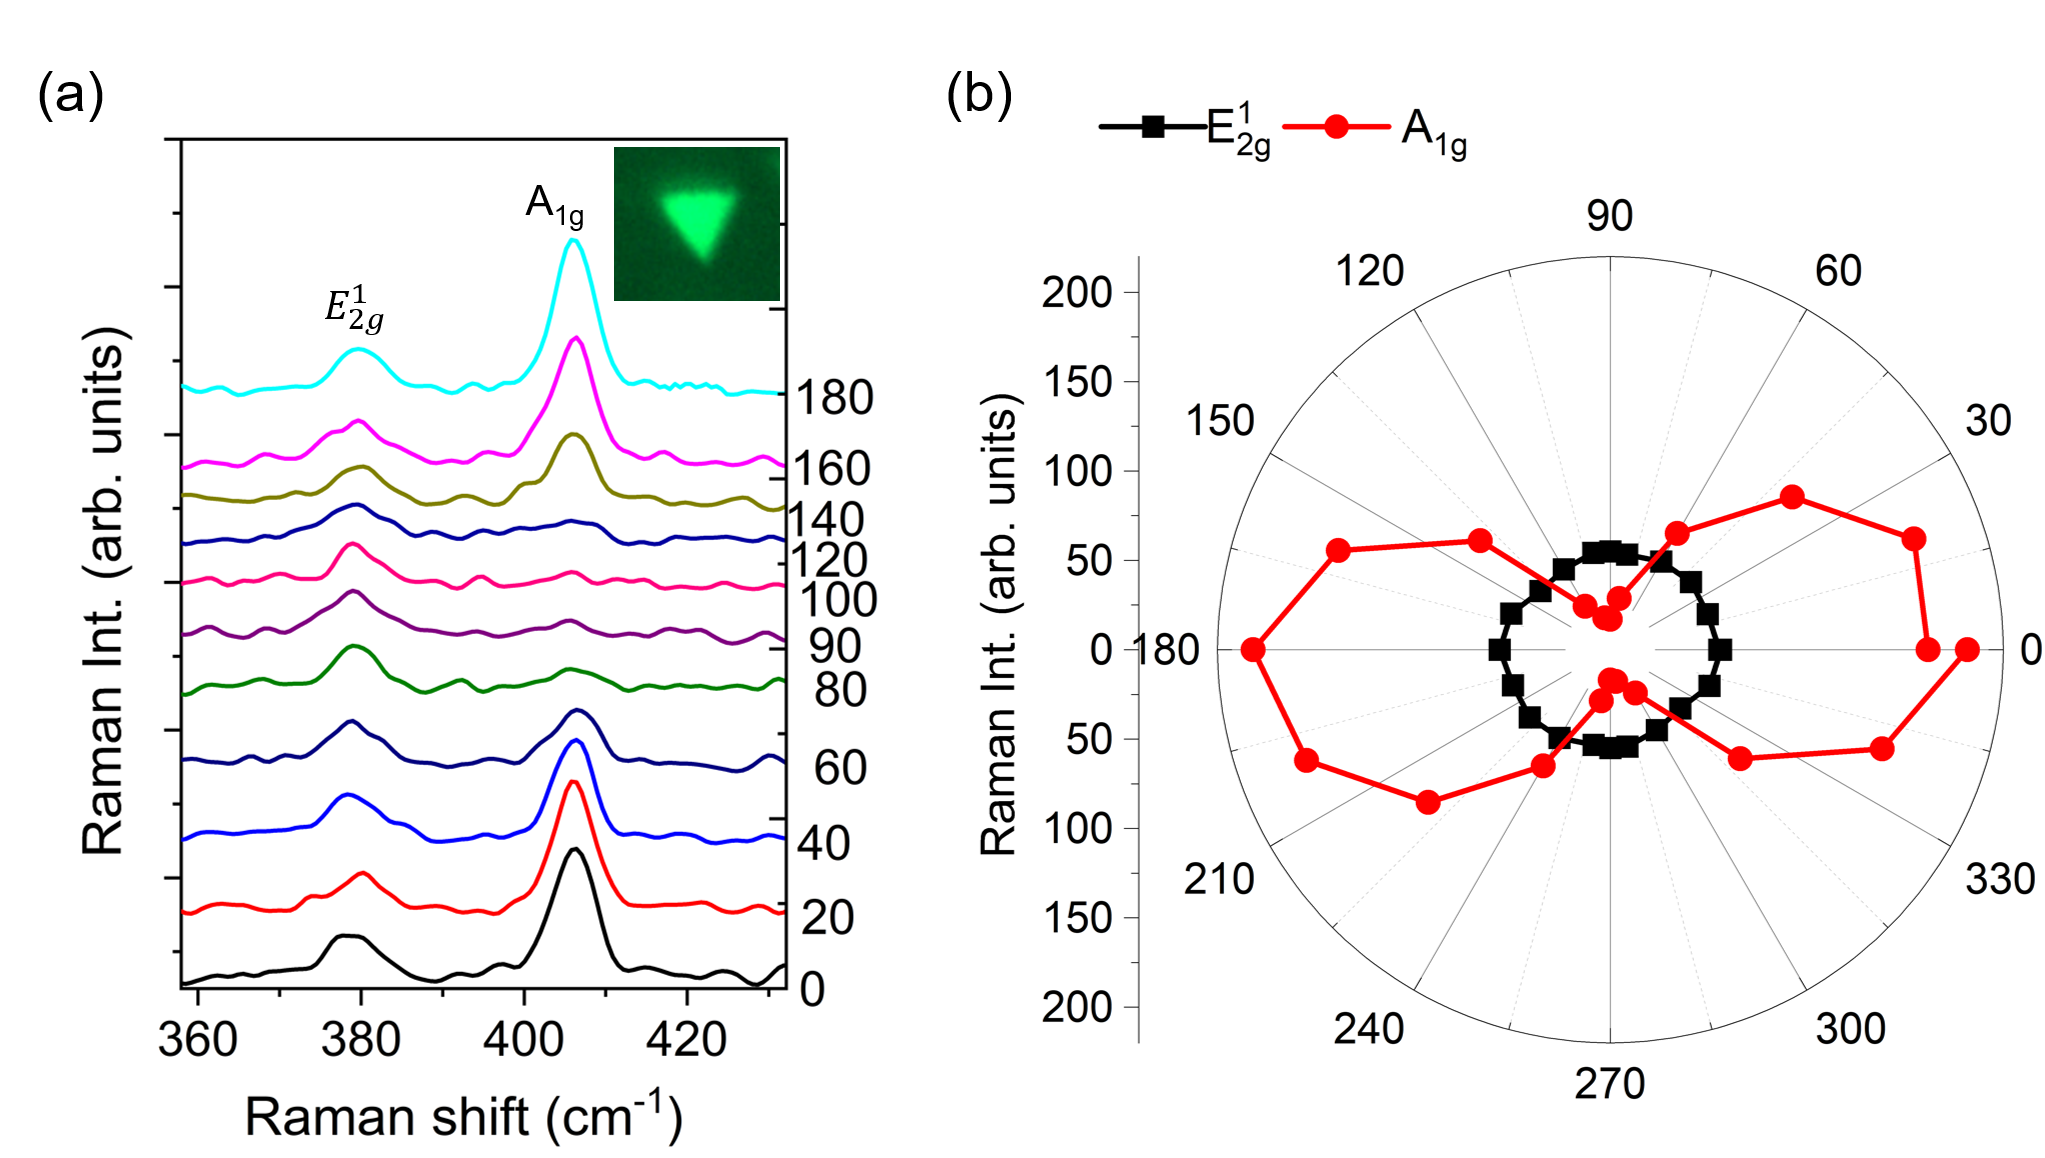
\includegraphics[width=0.9\linewidth]{Figures SI/Figure S3_polRaman triangle.png}
    \caption{\textbf{Isotropic Raman response of triangular MoS$_2$.}. (a) Angle-dependent Raman spectra collected while rotating the monolayer sample from $0^{\circ}$ to $180^{\circ}$. 
    (b) Polar plots of the Raman intensity for the $E^1_{2g}$ (black) and $A_{1g}$ (red) phonon modes. The $E^1_{2g}$ mode exhibits an isotropic response, whereas the $A_{1g}$ mode shows pronounced twofold anisotropy, characteristic of 2H-phase monolayer MoS$_2$.} 
    \label{fig:si_2D_Triangular MoS2}
\end{figure}

\newpage
\section{Supplementary Note 4} 
\textbf{Polarization resolved Raman mapping of MoS$_2$ nanoribbons and triangular MoS$_2$:}
\begin{figure}%[t]
    \centering 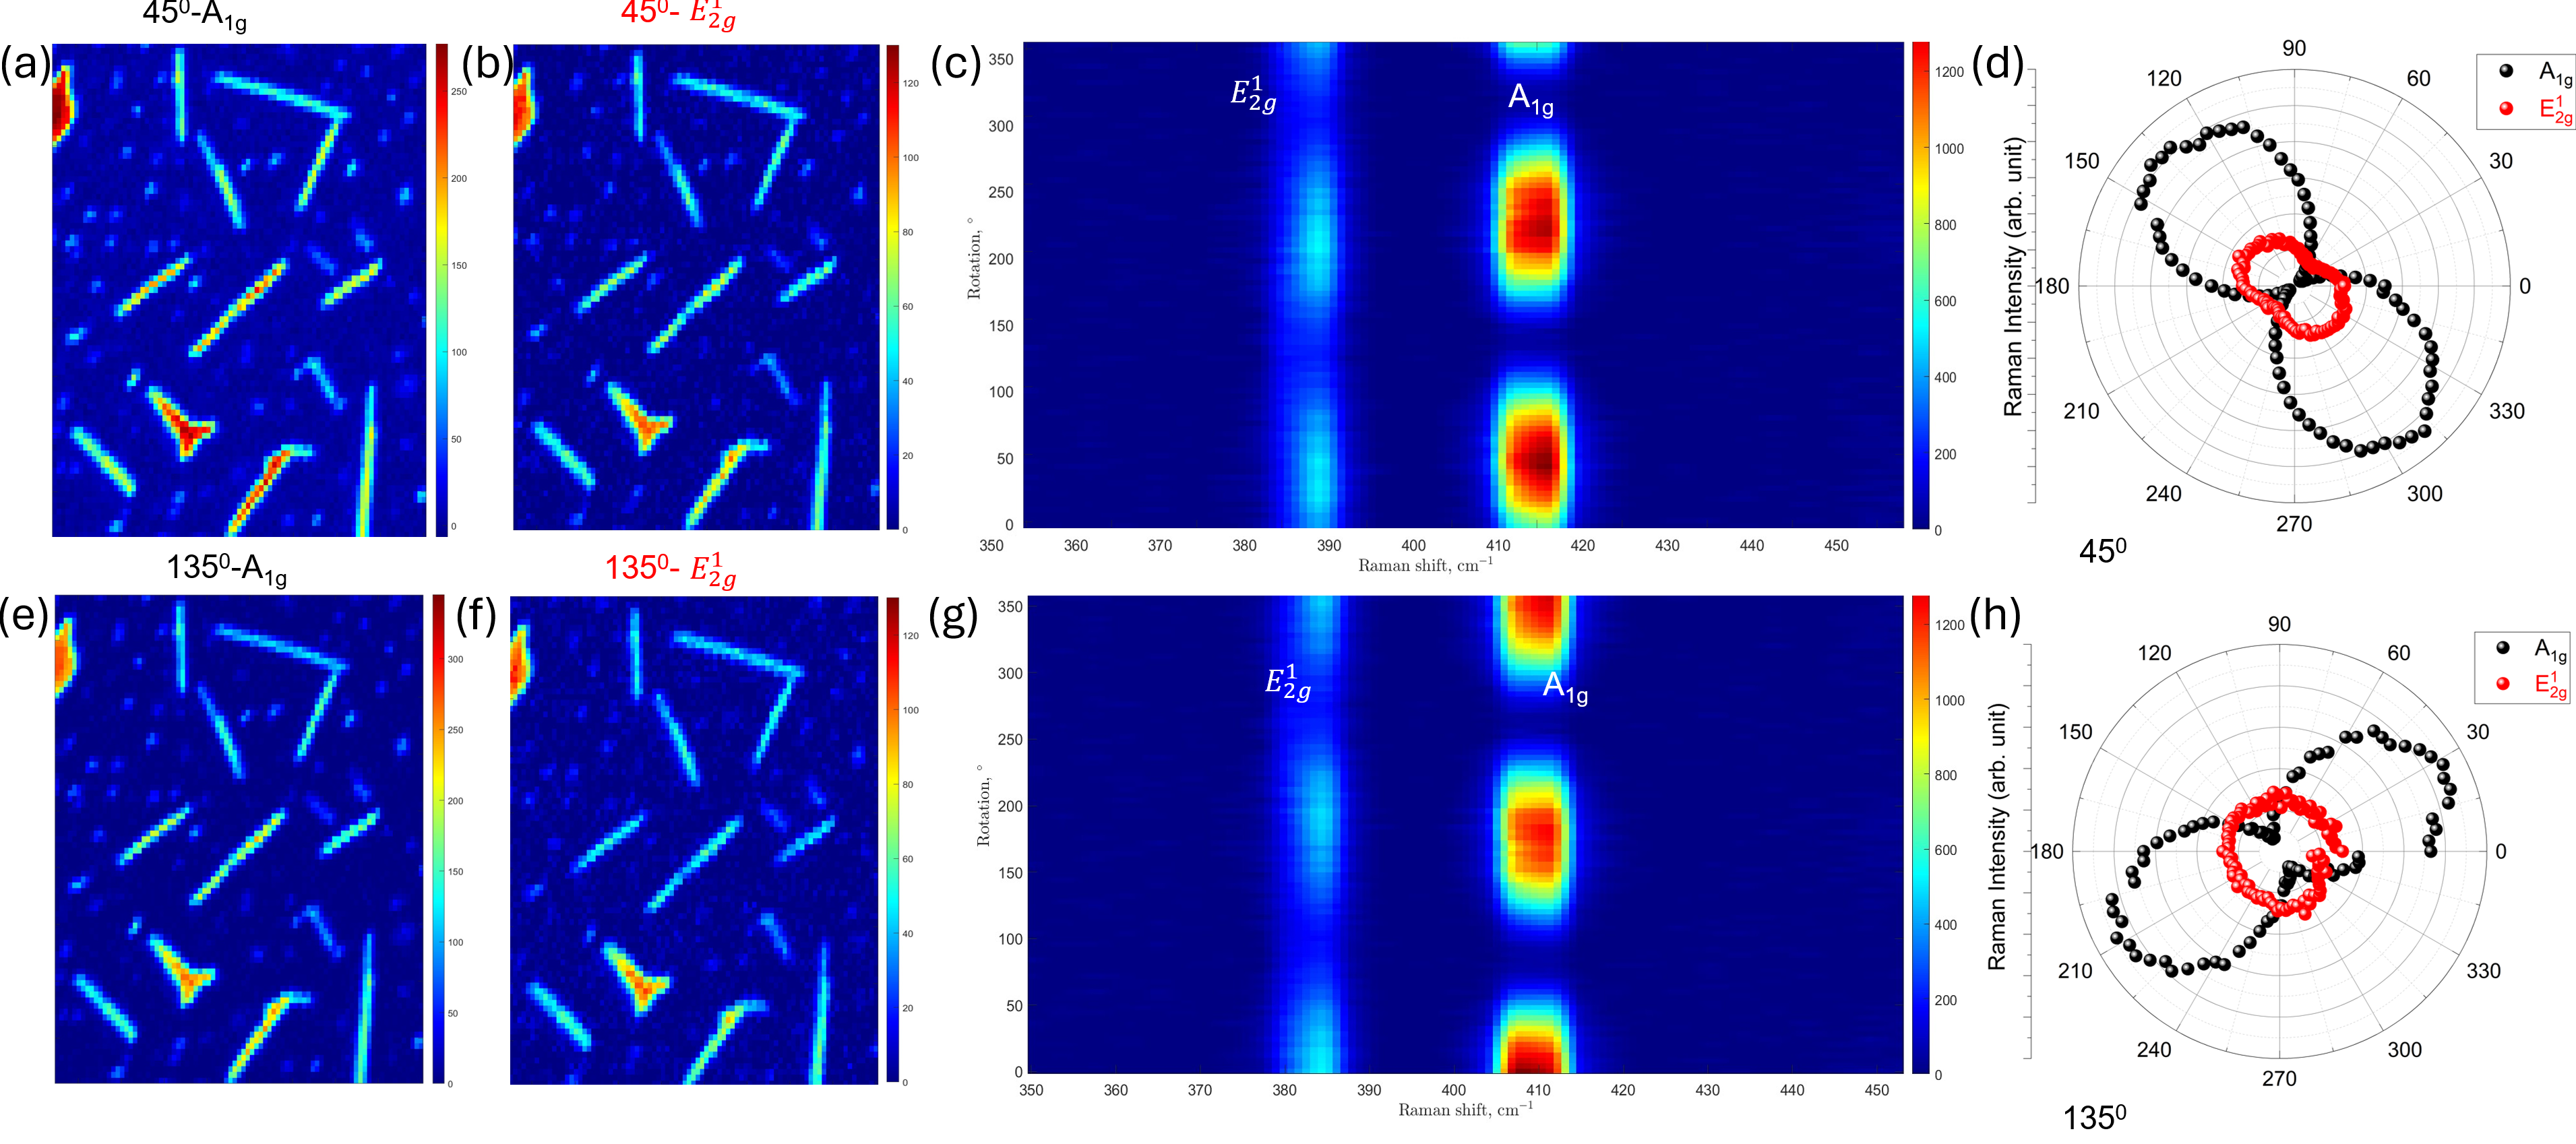
\includegraphics[width=1.0\linewidth]{Figures SI/Figure_S4_Polarization-resolved Raman mapping.png}
    \caption{\textbf{Polarization-resolved Raman mapping of MoS$_2$ nanoribbons.}
(a,b) Raman intensity maps of the A$_{1g}$ and E$^1_{2g}$ modes acquired under an incident
polarization of $45^\circ$, with strong spatial contrast across individual nanoribbons.
(c) Angle-resolved Raman contour maps showing the evolution of the E$^1_{2g}$ and A$_{1g}$ (d) Corresponding polar plots of the Raman intensities for the A$_{1g}$ and E$^1_{2g}$ modes 
extracted from the $45^\circ$ rotational scans
(e,f) Raman maps measured under an incident polarization of $135^\circ$. 
(g) Angle-resolved Raman contour maps showing the evolution of the E$^1_{2g}$ and A$_{1g}$ at $135^\circ$ (h) Corresponding polar plots of the Raman intensities for the A$_{1g}$ and E$^1_{2g}$ modes 
extracted from the rotational scans.
}
\label{Fig_SI_4}
\end{figure}
Figure~\ref {Fig_SI_4}a presents the polarization dependent Raman response of MoS$_2$ nanoribbons, measured under cross polarized excitation and detection geometries at $45^\circ$ and $135^\circ$. Panels (a,b,e,f) show spatial Raman maps of the A$_{1g}$ and E$^{1}_{2g}$ modes, revealing pronounced intensity variations as a function of both crystallographic orientation and polarization. The nanoribbons exhibit strong polarization contrast, where the Raman intensity of the out-of-plane A$_{1g}$ mode and the in-plane E$^{1}_{2g}$ mode both change significantly between the $45^\circ$ and $135^\circ$ configurations. 
Such behavior reflects the intrinsic structural anisotropy of  MoS$_2$ nanoribbons. Their reduced lateral width induces symmetry breaking, modified Raman tensor elements, and strain gradients along the ribbon axis, all of which enhance polarization selectivity. The corresponding angle resolved Raman maps in Figure~\ref {Fig_SI_4}c,g further show that the E$^{1}_{2g}$ mode exhibits an asymmetric and highly angle dependent intensity profile, whereas the A$_{1g}$ mode displays even larger modulation amplitude with a pronounced two-lobed pattern. These observations confirm a substantial in plane anisotropy arising from the  geometry and possible 3R-like stacking distortions generated during liquid-phase assisted growth.

The polar plots in Figure~\ref {Fig_SI_4} d,h quantify the angular dependence of both Raman active modes. The degree of polarization, calculated as $(I_{\parallel}-I_{\perp})/(I_{\parallel}+I_{\perp})$, yields distinctly non-zero values for both A$_{1g}$ and E$^{1}_{2g}$ modes in nanoribbons, unambiguously demonstrating anisotropic vibrational response. The strong modulation of the A$_{1g}$ mode, in particular, is consistent with symmetry breaking and non-uniform interlayer coupling within narrow MoS$_2$ ribbons.
For comparison, similar measurements performed on large area monolayer triangular MoS$_2$ flakes display negligible angular dependence for the in-plane E$^{1}_{2g}$ mode and only weak modulation for the A$_{1g}$ mode. This isotropic behavior is expected for monolayer MoS$_2$ in the 2H phase, where the hexagonal symmetry enforces polarization independent Raman response.
The clear contrast between the highly anisotropic nanoribbons and the nearly isotropic triangular domains highlights the role of reduced dimensionality in governing polarized Raman scattering. In 1D nanoribbons, strain, edge termination, and local symmetry breaking modify the Raman tensor elements, giving rise to the strong anisotropy observed in both modes. In contrast, 2H-phase triangular monolayers retain full in plane symmetry and therefore show minimal polarization sensitivity. These results demonstrate that polarized Raman spectroscopy serves as a powerful diagnostic tool to distinguish between  anisotropic MoS$_2$ nanostructures and their isotropic 2D counterparts.

\section {Supplementary Note 5} 
\textbf{Width dependent excitonic anisotropy in MoS$_2$ nanoribbons:} To further support the result obtained in ~Figure~\ref{fig:polar_reflect} of the main text, we performed
polarization resolved differential reflectance measurements on different size of nanoribbon and studied. Here the additional MoS$_2$
nanoribbon with a thickness of $\sim 30.2$~nm but a significantly larger width of
$\sim 600$~nm Figure~\ref{fig:si_5_width_dependent_anisotropy}\,a. Despite its comparable thickness to the 
ribbon studied in ~Figure~\ref{fig:polar_reflect} ($\sim 29.1$~nm) in the main text, the wider geometry produces a markedly 
different optical response. In particular, the excitonic resonances (Peaks~1 and~2) 
display almost isotropic polarization dependence, and the third low-energy FP mode 
exhibits only a weak signature of the FP cavity mode. This stands in
contrast to the narrower $\sim 400$~nm ribbon in ~Figure~\ref{fig:polar_reflect}, in the main text peaks 2 and 3 show clear twofold anisotropy and the FP mode is strongly enhanced. These observations indicate that lateral optical confinement plays a decisive role in establishing anisotropic exciton--photon coupling in  MoS$_2$ nanoribbons. When the width increases, the effective in plane cavity length becomes too large to  support strong FP coupling, leading to suppressed anisotropy and spectral redshifting of the FP resonance. Conversely, narrower ribbons confine the optical field more efficiently, enabling pronounced angular modulation of both excitonic and FP coupled features. This width dependence complements further confirms that the emergence of strong excitonic anisotropy in MoS$_2$ nanoribbons is a combined consequence of reduced dimensionality, and lateral photon confinement.\cite{BattulgaacsPhotonics}
\begin{figure}%[t]
    \centering
    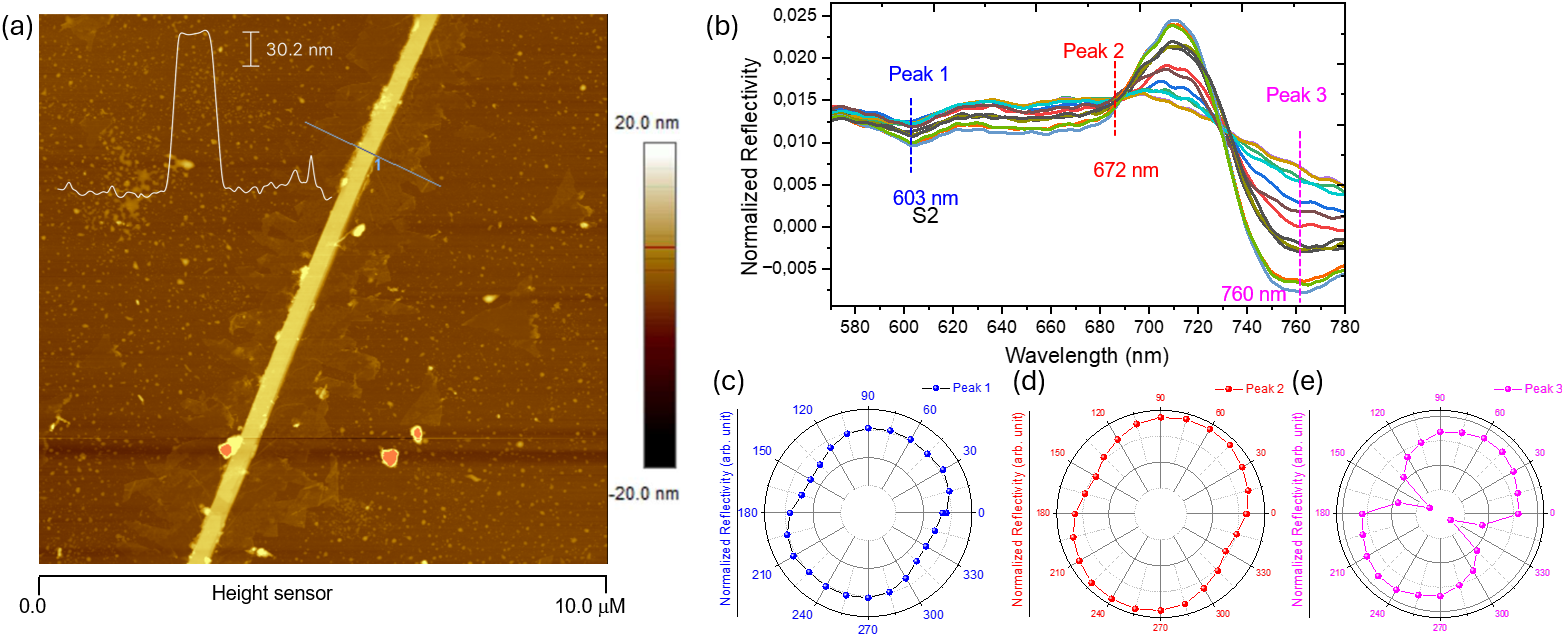
\includegraphics[width=1.0\linewidth]{Figures SI/Figure_S5_Width Dependent Excitonic Anisotrop.png}
\caption{\textbf{Polarization-resolved differential reflectance of a narrower and thicker MoS$_2$ nanoribbon.}
(a) AFM image of the nanoribbon showing a thickness of $\sim$30.2\,nm. 
(b) Normalized differential reflectance spectra measured as a function of incident polarization angle, revealing three optical resonances (Peak~1, Peak~2, and Peak~3). 
(c--e) Polar plots of the angular dependence of the three resonances. 
The broader nanoribbon exhibits modest anisotropy in Peak~1 and Peak~2, while Peak~3 (Fabry--Pérot-assisted mode) shows a stronger twofold modulation, reflecting the combined influence of ribbon geometry, thickness, and light matter coupling.} 
    \label{fig:si_5_width_dependent_anisotropy}
\end{figure}
\begin{figure}%[t]
    \centering 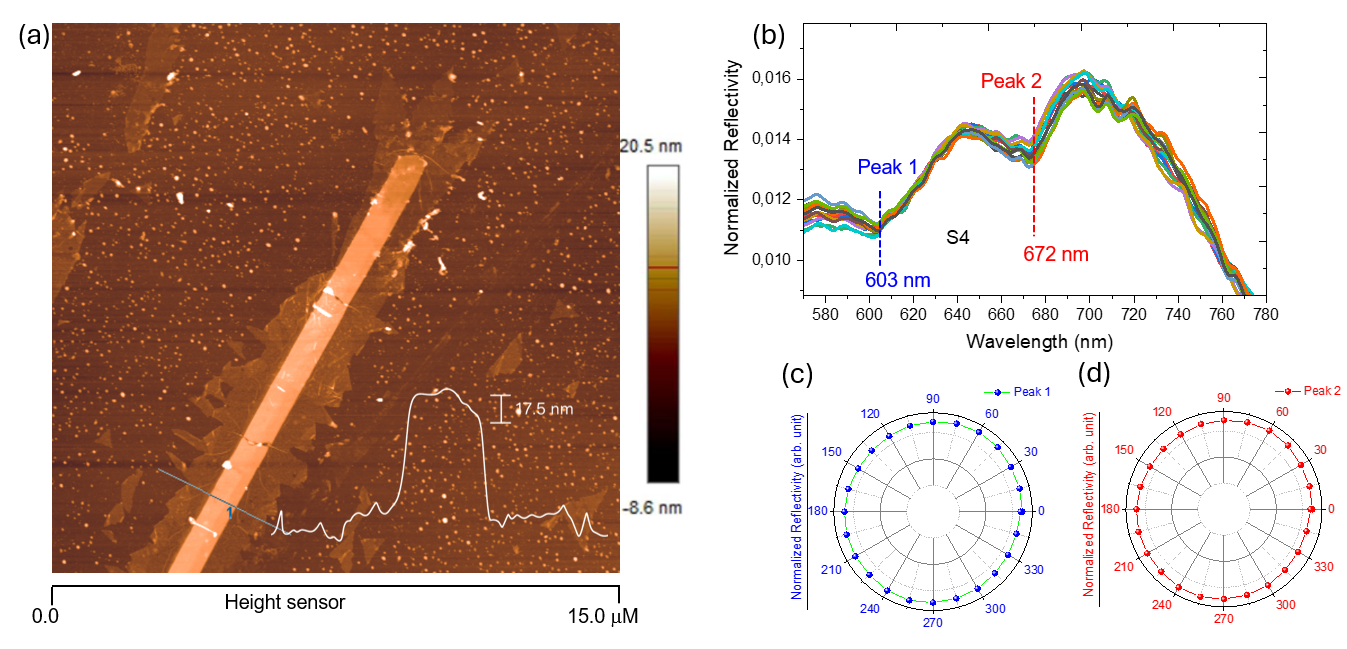
\includegraphics[width=1.0\linewidth]{Figures SI/Figure_S6_Width Dependent Excitonic Anisotropy.png}
    \caption{\textbf{Polarization-resolved differential reflectance of a wider MoS$_2$ nanoribbon}. (a) AFM image of the nanoribbon, showing a thickness of $\sim$17.5\,nm and a lateral width of $\sim$1\,$\mu$m.  (b) Polarization-dependent differential reflectance spectra measured while rotating the incident polarization from $0^{\circ}$ to $360^{\circ}$. In this relatively wide ribbon, only two optical resonances are observed at 603\,nm and 672\,nm (peak\,1 and peak\,2), while the Fabry--Pérot assisted mode that appears in narrower ribbons is absent.  (c, d) Polar plots of the angular dependence of peak\,1 and peak\,2 respectively. } \label{fig:si_6_width_dependent_anisotropy_wider}
\end{figure}

To further clarify the role of geometric confinement on the optical response, we investigated a MoS$_2$ nanoribbon with a relatively large width of $\sim 1~\mu$m and a smaller thickness of $\sim 17.5$ nm Figure~\ref{fig:si_6_width_dependent_anisotropy_wider}. In contrast to the narrower and thicker nanoribbons discussed previously, this structure exhibits only two excitonic resonances at 603 nm and 672 nm (Peaks 1 and 2), while the FP cavity mode observed in confined nanoribbons is absent. The absence of the FP resonance can be attributed to the combined effects of reduced vertical optical thickness and weak lateral confinement. Formation of FP-assisted modes requires sufficient cavity thickness to support standing optical waves together with lateral confinement that enhances photon localization along the ribbon axis. In the present ribbon, the small thickness ($\sim$17.5 nm) limits the effective optical cavity length, while the large lateral width suppresses in-plane confinement. As a result, the optical field cannot form a stable cavity resonance, and the spectrum is dominated solely by the intrinsic excitonic transitions. These results further confirm that the emergence of the FP-assisted resonance in MoS$_2$ nanoribbons requires a cooperative interplay between ribbon thickness and lateral confinement. Only when both conditions are satisfied, as in the narrower nanoribbons discussed in the main text, does strong cavity–exciton coupling appear, leading to the additional anisotropic resonance.

To further explain the role of lateral confinement on the optical anisotropy of  MoS$_2$ nanoribbons, we performed polarization-dependent differential 
reflectance spectroscopy on a narrower ribbon with a thickness of  $\sim 22.5$ nm and a lateral width of $\sim 300$ nm Figure~\ref{fig:si_5_width_dependent_anisotropy_narrower}. In contrast to the wider ribbons presented in the main text, this highly confined 
structure exhibits three well defined resonant features at 603 nm, 652 nm, and 681 nm (Peaks 1–3), all of which display strong and systematic angular modulation. The emergence of the third resonance (Peak 3) and its clear twofold anisotropy indicate the formation of an enhanced FP cavity along the confined ribbon axis. As the ribbon width decreases, the lateral optical path length becomes comparable to half wavelength multiples of the excitonic transition energies. This condition favors the formation of guided FP cavity modes whose phase-matching couples efficiently to the intrinsic excitonic resonances. Consequently, FP modes become more pronounced and shift towards shorter wavelengths (higher energies), appearing closer to the intrinsic B exciton. Such behavior is expected for dielectric nanoresonators with reduced lateral dimensions, where modified boundary conditions compress the optical field and shift cavity resonances. In addition, Peak 2 (the B exciton) exhibits a noticeable blue shift relative to wider nanoribbons. This shift arises from enhanced lateral confinement, which modifies the effective dielectric screening and strengthens Coulomb interactions, thereby increasing the exciton binding energy. The resulting renormalization drives the B exciton to higher energy, consistent with the trend expected when transitioning from a quasi-2D layer to an increasingly anisotropic geometry. Polar plots of the three resonances Figure~\ref{fig:si_5_width_dependent_anisotropy_narrower} c–e reveal pronounced twofold symmetry for all modes, significantly stronger than that observed in wider nanoribbons. This confirms that the narrowing of the ribbon enhances the directional dependence of light
matter coupling by restricting exciton transport and optical field distribution along a single dominant axis. These findings provide compelling evidence that the optical anisotropy in MoS$_2$ nanoribbons is highly tunable through geometric confinement, and that new FP-assisted resonances naturally emerge as the system approaches the quasi-1D limit.
\begin{figure}%[htb]
    \centering 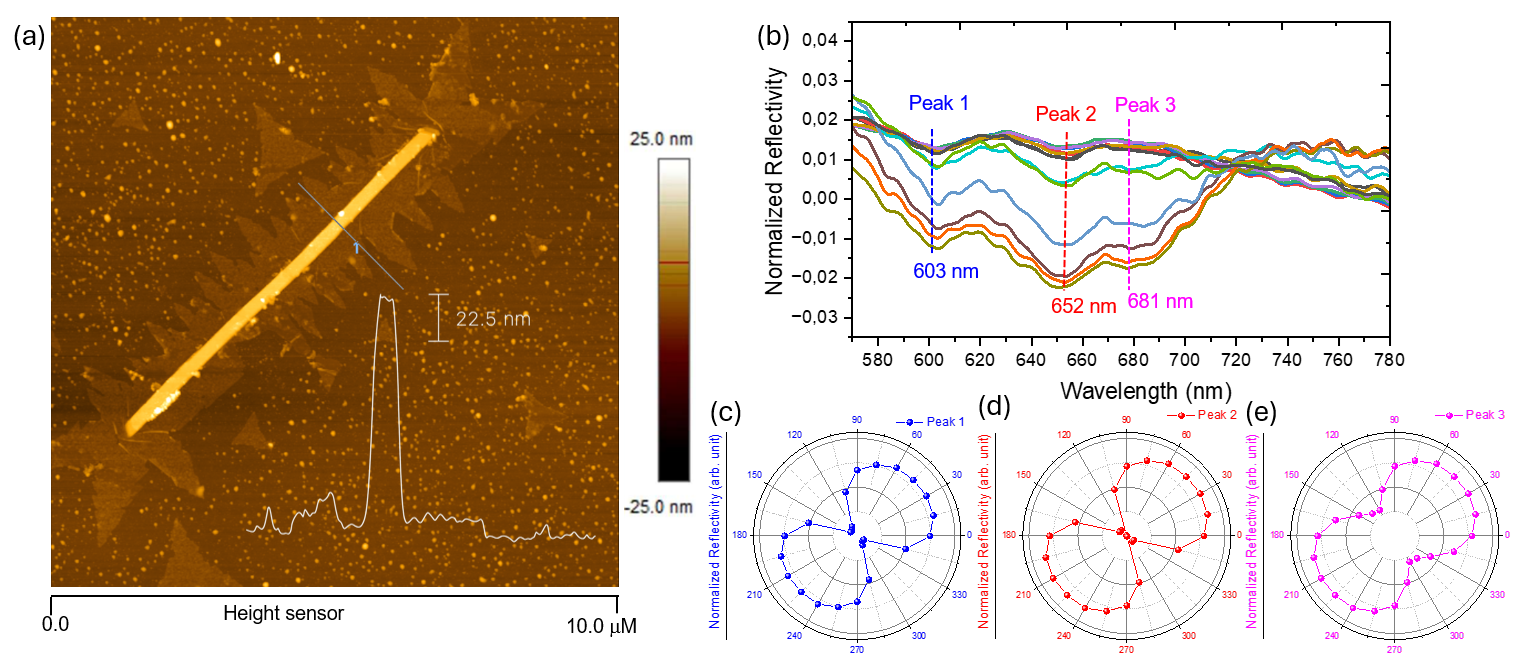
\includegraphics[width=1.0\linewidth]{Figures SI/Figure_S7_Width Dependent Excitonic Anisotropy.png}
    \caption{\textbf{Polarization-resolved differential reflectance of a narrower and thinner MoS$_2$ nanoribbon}. (a) AFM image of a nanoribbon with a thickness of $\sim22.5$ nm and a width of $\sim300$ nm. (b) Differential reflectance spectra measured as a function of incident polarization, showing three clear resonances at 603 nm, 652 nm, and 681 nm. (c–e) Polar plots of the angular dependence of the three resonances. The reduced ribbon width leads to pronounced anisotropy in all modes and the emergence of a strongly polarization-sensitive Fabry–Pérot (FP) resonance that shifts toward the excitonic energies due to enhanced lateral confinement and stronger cavity–exciton coupling.} 
\label{fig:si_5_width_dependent_anisotropy_narrower}
\end{figure}
\newpage

\end{itemize}
\end{suppinfo}
\newpage 

\end{document}